% Design & Implementation

\chapter{Design and Implementation} 

\label{Chapter5} 

\lhead{Chapter 5. \emph{Design \& Implementation}} 

In this chapter we go over the design and implementation process of the project. We describe various choices we made, justifying them in the context of our objectives. 

First, we describe our solution to the mood detection problem. We attempt that by trying to determine which musical features are the most correlated to the AV values of the music's emotion. Having found the set of features that have the biggest impact on our perception of the emotions in the song, we train a neural network with data containing chosen features. This way we create a way of determining the arousal and valence values of any musical track. The system is later used in the implementation of our game. In addition to this, by investigating the impact of different parameters, we make sure out network has as good performance and accuracy as possible.

Next, we move on to main melody detection by looking at two algorithms - one using source separation based approach and the other using the salience based approach. We evaluate performance of both of them on data from recent pop culture to determine their performance and fitness in this project. In addition to this, we employ post processing to further modify the output of the chosen algorithm and smooth out the pitch contours, removing outliers that could interfere with the gameplay. Thanks to parametrising and applying the sliding median we are able to produce pitch coutours of different difficulty to play.

The next section describes our attempt to design and develop an automated music segmentation system. We investigate two different features -- Mel-frequency cepstral coefficients and harmonic pitch class profiles, to generate a self-similarity matrix and apply the convex non-negative matrix factorisation (C-NMF) to retrieve its decomposition matrices. Using those matrices, we then investigate two different ways of finding boundaries of a musical track. Finally, we describe our process of inventing a novel way of labelling segments of the song.

Last, but not least, we talk about the game itself, its architecture, flow of use and design choices made. We describe the algorithm for generating buttons that constitute the main part of the gameplay. We also detail the way we tie in the music analysis performed into the game to make the most of it.

\vspace{20pt}

\section{Mood Detection}

A common reason for engaging in listening to music is that it is an effective means of conveying and evoking emotions. Although they may be subjective, based in part on the listener’s cultural and musical background or preferences, there are common points in perceived emotion across different listeners based on the characteristics of the music \cite{vempala}. Several studies have attempted to predict emotion conveyed during music listening. In our approach, we decided to represent the emotion connected to the music using a two-dimensional space with valence on the x-axis and arousal on the y-axis, first proposed by R. E. Thayer \cite{Thayer}.

As we described in Section \ref{sec:emotionClass}, there is a relation between valence and arousal values for a musical track and the mood perceived by people. In essence, the high arousal is connected to how energetic the music is, whereas valence refers to how positive (or negative) the emotions in the track are. 

\vspace{10pt}

\subsection{Choice of Features}
Using Essentia library \cite{essentia}, we implemented an extractor to retrieve certain features from a song. We chose the features on the impact we expected them to have on the perceived mood of a musical piece:

\begin{description}

\item[average loudness] - describes dynamic range (the ratio between the largest and smallest possible values of the signal) of loundness. The values are rescaled into the [0, 1] interval on a per window basis - if 0, it means that the signal exhibits a large dynamic range, 1 corresponds to signal with little dynamic range. This could indicate the level of the arousal, with higher loudness implying higher arousal value. We believe this relation could be quite intuitive - sad or peaceful songs tend to be quiet whereas excited or angry emotions are usually linked to louder tracks or tracks that vary greatly in loudness.

\item[means and derivatives of variance of rates of silent frames] in a signal for thresholds of 20, 30 and 60db. We believe that the values could influence the arousal levels, as the more and the bigger the silent gaps, the sadder or more peaceful the track seems to be, implying the low arousal value. When examining multiple musical tracks, we noticed that the happier or angrier songs can also have such silent gaps, but they tend to be much shorter and less frequent.

\item[dynamic complexity] - is the average absolute deviation from the global loudness level estimate on the dB scale. It is related to the dynamic range and to the amount of fluctuation in loudness present in a recording. We believe this feature would have an impact on both examined values. However, similarly to the loudness level, arousal should be influenced more - as more dynamic songs (excited or angry) are more likely to suffer from loudness changes, whereas more phlegmatic ones (sad or peaceful) tend to keep the same dynamic complexity level.

\item[BPM] - beats per minute value according to detected beats. This feature should be correlated with the arousal level - intuitively, the faster the song, the more energetic it seems. 

\item[spectral centroid] - centroid statistics describing the spectral shape. It indicates where the ``centre of mass'' of the spectrum is. Perceptually, it has a robust connection with the impression of ``brightness'' of a sound - an indication of the amount of high-frequency content in a sound. Timbre researchers consider brightness to be one of the perceptually strongest distinctions between sounds, and formalise it acoustically as an indication of the amount of high-frequency content in a sound \cite{timber}. That is why we believe the spectral centroid might be related to both valence and arousal.

\item[spectral RMS] (root mean square) - in Physics, it is a value characteristic of a continuously varying quantity, such as a cyclically alternating electric current or a sound. It is obtained by taking the mean of the squares of the instantaneous values during its duration or a cycle. In audio processing, it is linked to the loudness of the sound. This is why we believe that it might have an impact on arousal, but we do not exclude its impact on valence.

\item[spectral energy] - the energy $E_{s}$ of a continuous-time signal $x(t)$ defined as: 
\begin{equation}
E{s}  =  \langle x(t), x(t)\rangle =  \int_{-\infty}^{\infty}{|x(t)|^2}dt
\end{equation}

Signal energy is always equal to the summation across all frequency components of the signal's spectral energy density. 
There have been some research focusing on relation between spectral energy and singing voice. In particular, in their paper \cite{spectralenergy}, Ferguson, Kenny and Cabrera were investigating the relation between the value and the experience of male singers. This makes for an interesting case worth considering in our research.

\item[mean and derivative of variance of beat loudness] -  spectral energy computed on beats segments of audio across the whole spectrum, and ratios of energy in 6 frequency bands. We suspect that the low value of the beat loudness could imply a low arousal as loud beats can be found in parts of song with higher energy.

\item[key and its scale] estimated key and its scale (major or minor) using Temperley’s profile. 
In music theory, the term key is used in many different and sometimes contradictory ways. A common use is to speak of music as being ``in'' a specific key, such as \textit{``in the key of C major or in the key of F\#''}. Sometimes the terms ``major'' or ``minor'' are appended, as \textit{``in the key of A minor''} or \textit{``in the key of B major''}.
Broadly speaking the phrase ``in key of C'' means that C is music's harmonic centre or tonic (the first degree of the scale, or the root of the scale). 
The terms ``major'' and ``minor'' further imply the use of a major scale or a minor scale. Thus the phrase \textit{``in the key of E major''} implies a piece of tonal music harmonically centred on the note E and making use of a major scale whose first note, or tonic, is E. 
We believe that those features can have an impact on both arousal and valence - songs performed in minor scale are traditionally connected to being sad, whereas the major scale is usually linked to positive emotions.

\item[scale and key of the chords] taken as the most frequent chord, and scale of the progression, whether major or minor. Scale commonly known to have a big influence on our perception on music \cite{keys}. It seems to be mostly the result of cultural conditioning as when people listen to tunes, they rely heavily on their memory. Such constant stimulus to our musical memory helps to generate expectations of what might come next in a tune or preserve the sound - emotion relation.

\item[mean ZCR] (zero-crossing rate) - the rate of sign-changes along a signal, i.e., the rate at which the signal changes from positive to negative or back. This feature has been used heavily in music information retrieval, being a key feature to classify percussive sounds. We believe it could be related to the arousal value. Music has a fairly normal distribution of frames with lower and higher zero-crossing rates. Speech however displays a much more skewed distribution. This could have an impact on songs where the vocals are quite rapid and energetic, for example rap music, and therefore might have a significant impact on mood recognition in our system.
ZCR is defined formally as: 
\begin{equation}
ZCR = \frac{1}{T-1} \sum_{t=1}^{T-1} {{\mathbb I}\left\{{s_t s_{t-1} < 0}\right\}}
\end{equation}
where $s$ is a signal of length $T$ and the indicator function  ${{\mathbb I}\left\{{A}\right\}}$  yields 1 if $A$ is true, 0 otherwise.

\item[pitch salience of a spectrum] - given by the ratio of the highest auto correlation value of the spectrum to the non-shifted auto correlation value.  Unpitched sounds (non-musical sound effects) and pure tones have an average pitch salience value close to 0 whereas sounds containing several harmonics in the spectrum tend to have a higher value. We think the value could have an effect on both the valence and arousal as pitch salience is often described as the probability of noticing a tone or clarity or strength of tone sensation.

\item[mean and derivative of variance of sensory dissonance] (to distinguish from musical or theoretical dissonance) of an audio signal given its spectral peaks. Sensory dissonance measures perceptual roughness of the sound and is based on the roughness of its spectral peaks. Given the spectral peaks, the algorithm estimates total dissonance by summing up the normalised dissonance values for each pair of peaks. These values are computed using dissonance curves, which define dissonance between two spectral peaks according to their frequency and amplitude relations. Dissonance could be related to low valence.

\end{description}

\begin{figure}[h]
	\centering
   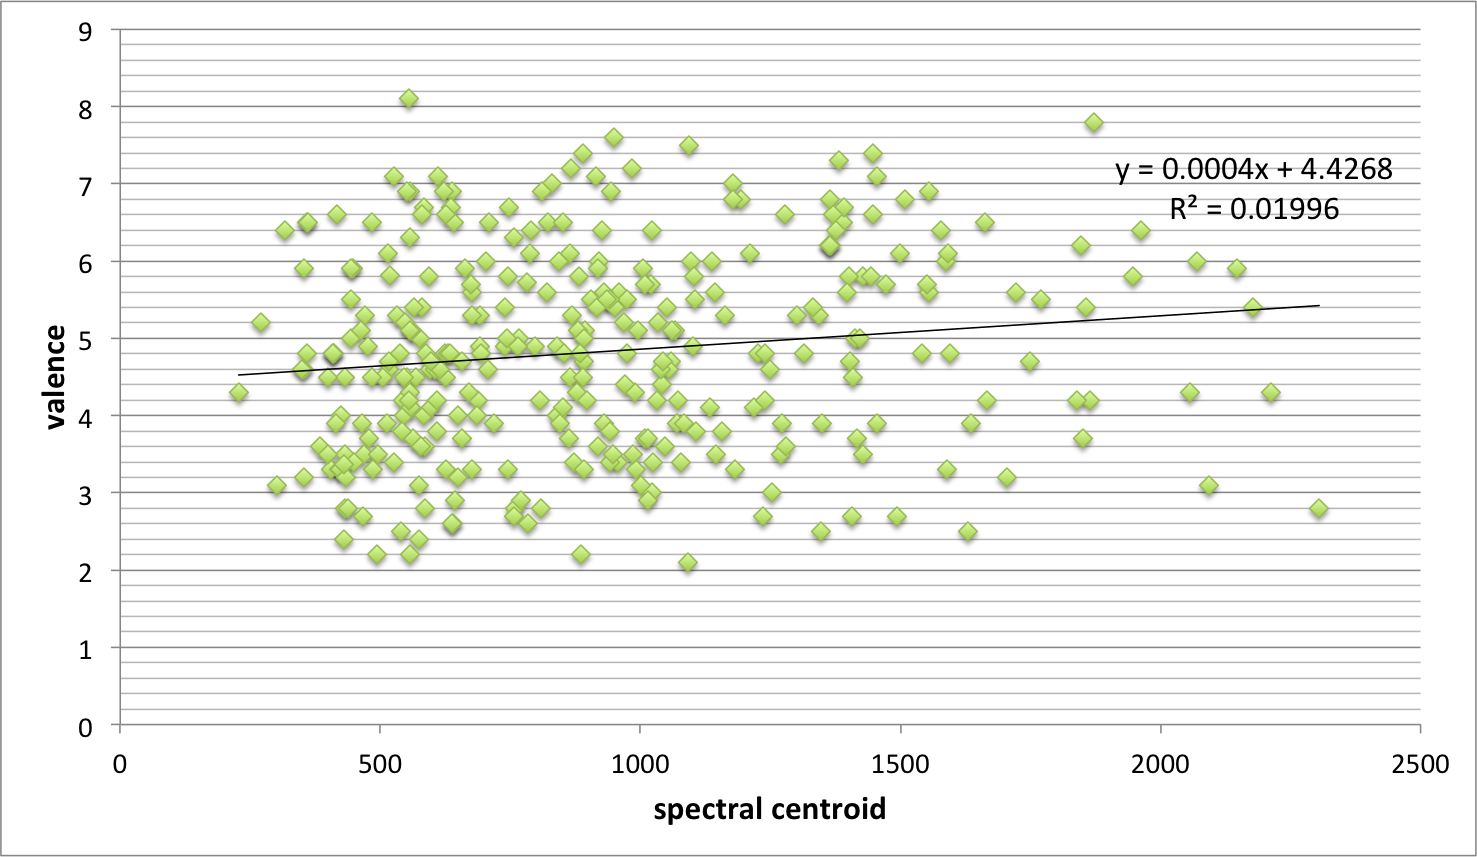
\includegraphics[width=0.7\textwidth]{Figures/spectralcentroid-valence}
\caption{A graph representing a correlation between spectral centroid and valence values.}
\label{fig:bivariate-valence}
\end{figure}


\begin{figure}[h]
	\centering
   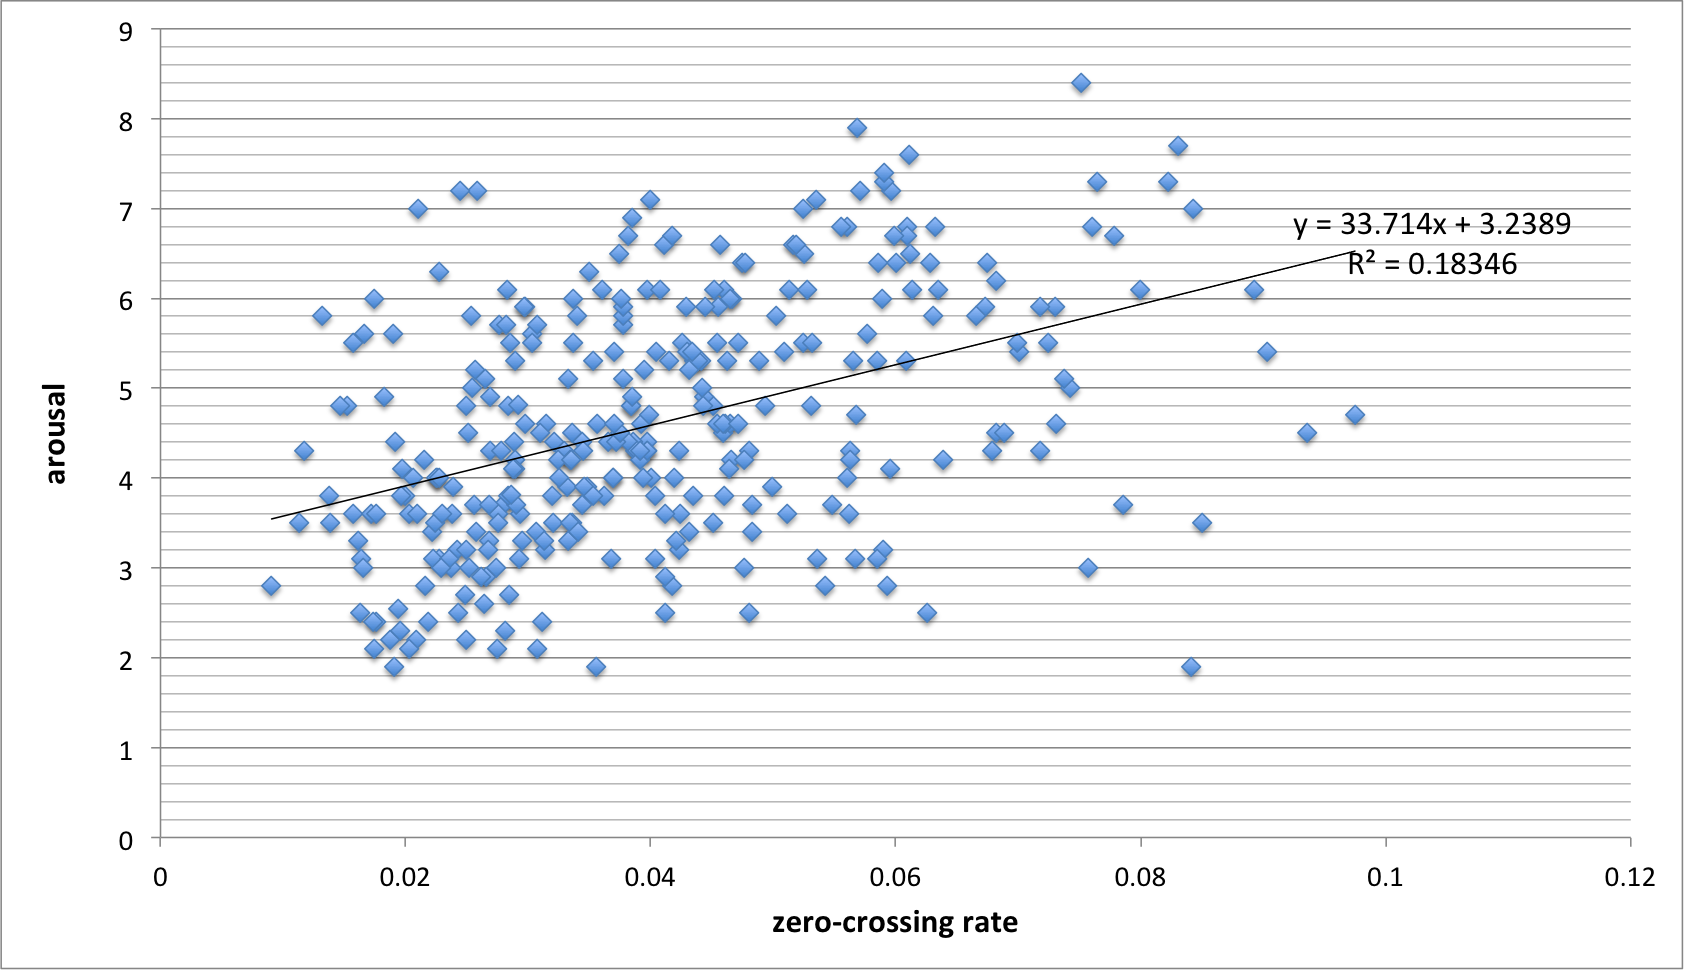
\includegraphics[width=0.7\textwidth]{Figures/zerocrossing-arousal}
 \caption{A graph representing a correlation between zero-crossing rate and arousal values.}
\label{fig:bivariate-arousal}
\end{figure}


\vspace{10pt}

\subsection{Correlation Between Features and Mood Perception}

In our exploration we decided to base our research on data collected in ``1000 Songs for Emotional Analysis of Music'' music library \cite{1000songs}, to avoid personal bias in assessing the mood of the song. The songs in the dataset were annotated by more than 300 crowdworkers on Amazon Mechanical Turk. Each song was annotated for arousal and for valence separately.

As a first step towards understanding the pattern by which audio features might account for emotion ratings, we conducted correlational analyses between features and mean valence/arousal ratings from the data set. We performed a bivariate correlation analysis with the valence/arousal ratings as the dependent variable, and each of the 22 features as the explanatory variable. Example of the results we achieved can be seen in Figured \ref{fig:bivariate-valence} and \ref{fig:bivariate-arousal}, the rest are included in Section \ref{sec:bivariatediagram}, Appendix A, for reference. 

We found significant correlation between \textbf{valence} and derivative of variance and mean \textit{silence60}, derivative of variance of \textit{silence30, dynamic complexity, spectral centroid, spectral RMS, spectral energy, zero-crossing rate, pitch salience}, and both mean and derivative of variance (dvar) of \textit{dissonance}. 

For \textbf{arousal}, we noticed correlation with \textit{spectral centroid, pitch salience, zero-crossing rate}, both mean and dvar of  \textit{silence60, spectral energy}, mean \textit{dissonance} and \textit{dynamic complexity}. 

Values of all the features were then normalised between 0 and 1 to prepare them for the neural network training. 

\begin{wrapfigure}{l}{0.5\textwidth}
  \vspace{-30pt}
  \begin{center}
    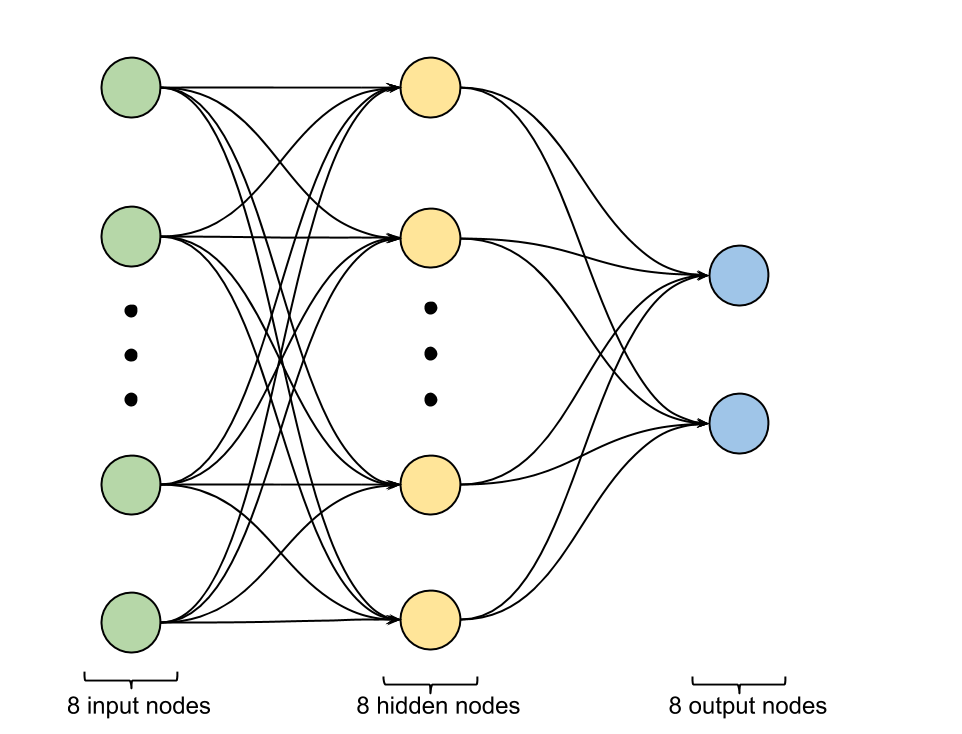
\includegraphics[width=0.5\textwidth]{Figures/myANN}
  \end{center}
  \caption{A diagram depicting the structure of our artificial neural network for mood detection.}
\label{fig:finalnetwork}
\end{wrapfigure}

\vspace{10pt}

\subsection{Neural Network for Mood Prediction}

Our goal was to train the network to predict mean participant valence and arousal values for musical excerpts.
 
Our network implementation was a supervised, feedforward network with backpropagation. 
The input consisted of normalised values of 8 features:
\textit{spectral centroid, pitch salience, zero-crossing rate, silence60 mean, loudness, mean dissonance, dynamic complexity} and \textit{spectral energy}. 
The network had two outputs - arousal and valence.

As all the training data was normalised, the input and output values were within a range of 0 to 1. The training set consisted of 50 input and output arrays. Each input array had 8 values, one per audio feature, and its corresponding output array had the two desired arousal and valence values.

The network’s task was to provide the valence and arousal values based on the 8 audio features. The output values fell within a range of 0 to 1. Since desired outputs were average valence/arousal ratings provided by participants on a scale from 0 to 10 inclusive, the network outputs were rescaled back. The training set consisted of 50 input and output arrays. The connection weights from input to the hidden nodes and from hidden nodes to the output ones were initialised to random numbers. 

The network was built, trained, and tested using the PyBrain \cite{pybrain} Python library for neural network implementation. 

Hidden neurons are the neurons that are neither in the input layer nor the output layer. Using additional layers of hidden neurons enables greater processing power and system flexibility at the cost of additional complexity in the training algorithm. Having too many hidden neurons can be thought of as a system of equations with more equations than there are free variables: the system is over specified and incapable of generalisation. Having too few hidden neurons, conversely, can prevent the system from properly fitting the input data, and reduces the robustness of the system.

We trained our network for 1000 epochs with many different sizes of the hidden layer and default values for all the other parameters. The performance based on that can be seen in Table \ref{table:rsmetable}.


\begin{table}
\begin{center}
\begin{tabular}{| c | l | l | l | l |} \hline 
  No. of Nodes & RMSE 1 & RMSE 2 & result 1 & result 2  \\ \hline \hline
  1 & 0.0727638 &  0.0740583  & 0.0998089  & 0.0978822   	\\ \hline
  2 & 0.0717966 &  0.0709793  & 0.1130468  & 0.1124054    	\\ \hline
  3 & 0.0722213 &  0.0733605  & 0.1554125  & 0.0948397   	\\ \hline
  4 & 0.0702014 &  0.0699922  & 0.1026024  & 0.1153731  	\\ \hline
  5 & 0.0659433 &  0.0693361  & 0.1165588  & 0.1042320		\\ \hline
  6 & 0.0722427 &  0.0751383  & 0.1422484  & 0.1188432		\\ \hline
  7 & 0.0698701 &  0.0678483  & 0.0889542  & 0.1035373		\\ \hline
  8 & 0.0692459 &  0.0664240  & 0.1314129  & 0.1360981		\\ \hline
  9 & 0.0676911 &  0.0707275  & 0.1281395  & 0.1042317		\\ \hline
 10 & 0.0684399 & 0.0673887  & 0.1405055  & 0.1751565		\\ \hline
 15 & 0.0671656 & 0.0673142  & 0.1165631  & 0.1392658		\\ \hline
 20 & 0.0737978 & 0.0720621  & 0.1604241  & 0.1362109		\\ \hline
 50 & 0.0669456 & 0.0694139  & 0.1641328  & 0.1716036		\\ \hline
\end{tabular}
\caption{Table showing the root mean square error for training the network for given number of nodes in the hidden layer.}
\label{table:rsmetable}
\end{center}
\end{table}


\begin{figure}[b]
	\centering
   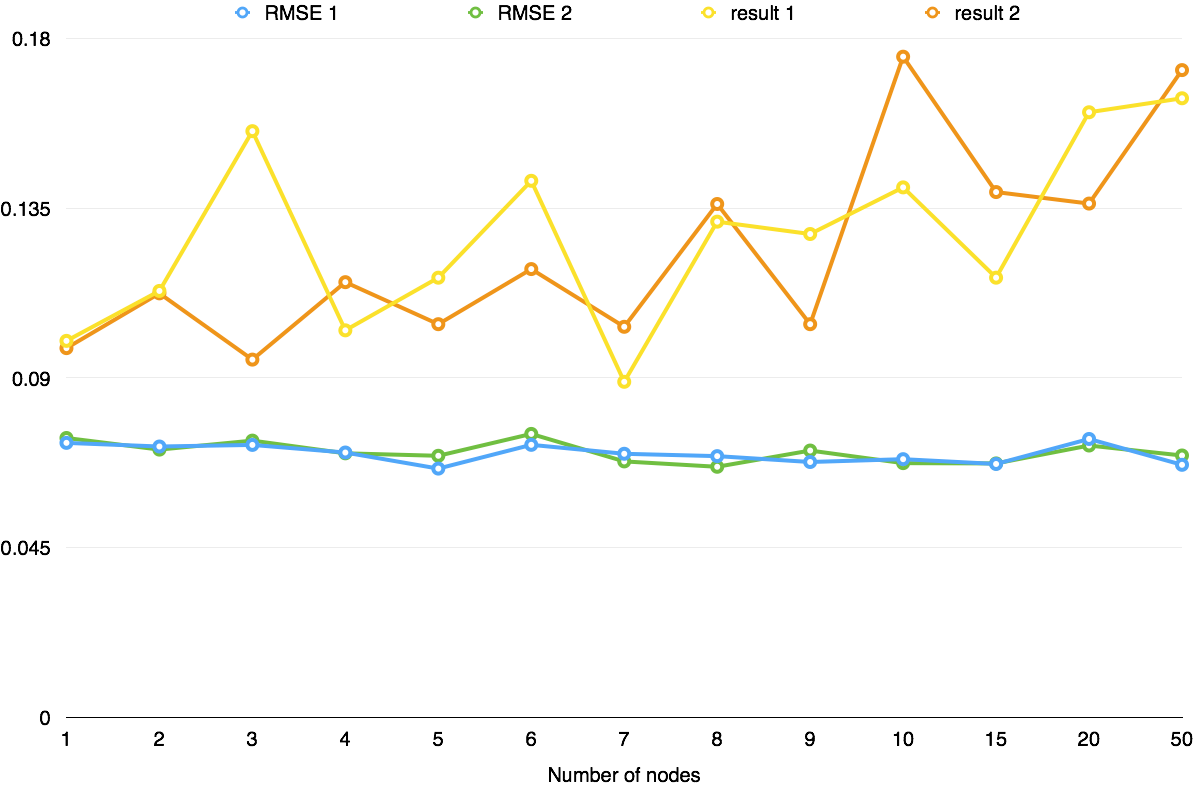
\includegraphics[width=0.7\textwidth]{Figures/nodesperf}
\caption{Data presented in Table \ref{table:rsmetable}, plotted on a diagram.}
\end{figure}

As we can see, the optimal solution is the one with 7 nodes in the hidden layer. Although the initial RMSE returned after training is not overall minimum, all the values -- so both the training ones and the ones after the evaluation, are local minimas and one of the minimal values overall. This decision can be justified by the fact that although for some cases we managed to achieve smaller RSME from the training, the network was in fact overfitting, and doing really well for the already known input, but worse for a new one.
To avoid overfitting the network, we kept the number of hidden units equal to the number of input units. 

\begin{table}
\begin{center}
\begin{tabular} {| c | l | l |} \hline
 Learning Rate & RMSE & result RMSE \\  \hline \hline
 0.3 		& 0.070797 	& 0.145788	\\ \hline
 0.25 	& 0.069934  	& 0.163193	\\ \hline
 0.2 		&  0.066799	& 0.155219	\\ \hline
 0.15		& 0.072422	& 0.104971	\\ \hline
 0.1 		& 0.068426	& 0.100719	\\ \hline
 0.05 	& 0.069596	& 0.097935	\\ \hline
 0.01 	& 0.068946	& 0.090954	\\ \hline
 0.005 	& 0.072402	& 0.130734	\\ \hline
 0.001 	&  0.079665	& 0.112620	\\ \hline
\end{tabular}
\caption{Table showing the root mean square error for training the network for given learning rate parameter value.}
\label{table:learningrate}
\end{center}
\end{table}

Having found the optimal number of nodes in the hidden layer, we moved on to find the learning rate parameter. Learning rate is essentially a training parameter that controls the size of weight and bias changes in learning of the training algorithm. In a standard backpropagation, too low a learning rate makes the network learn very slowly,whereas a learning rate that is too high makes the weights and objective function diverge, so there is no learning at all. 

We started our search by setting it to 0.3 and reducing it over time. The results we found can be found in Table \ref{table:learningrate}. As we can see, the optimal solution seems to be learning rate at value 0.001.


In the end, we came up with the network which can be seen on Figure \ref{fig:finalnetwork}.

\begin{figure}[h]
	\centering
   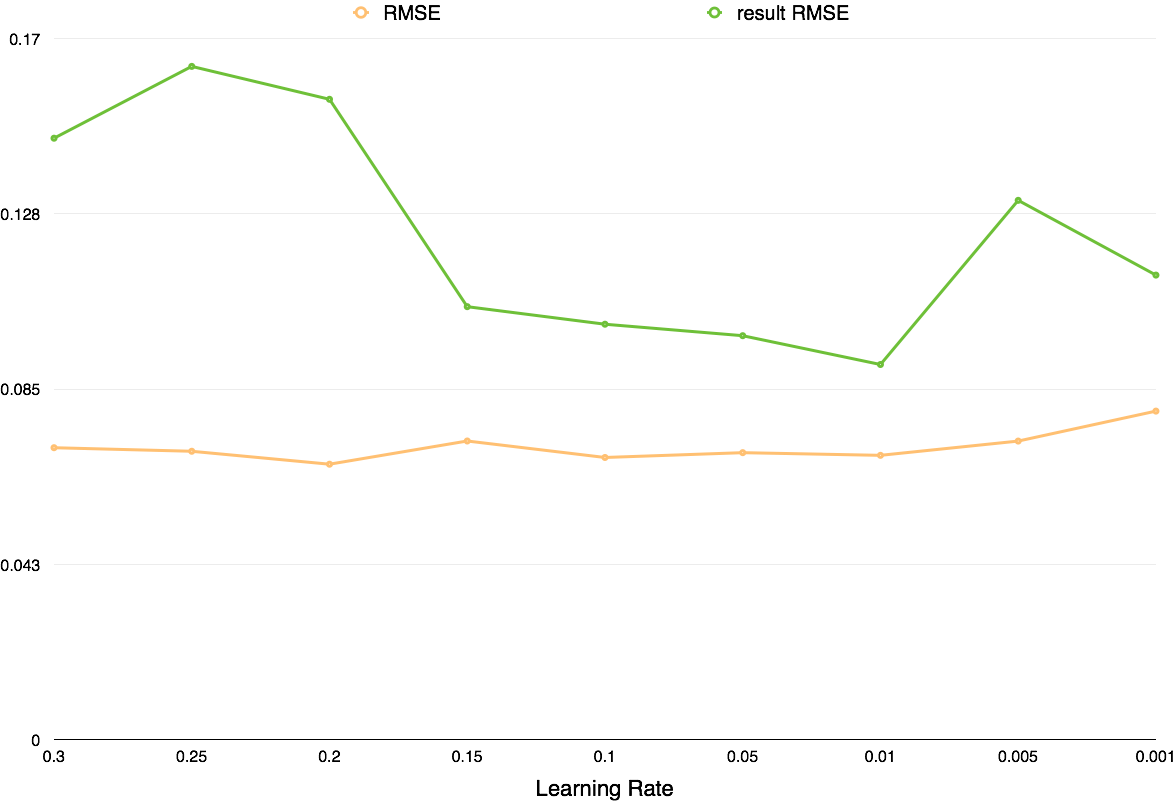
\includegraphics[width=0.7\textwidth]{Figures/learningrate}
\caption{Data presented in Table \ref{table:learningrate}, plotted on a diagram.}
\end{figure}

\vspace{20pt}

\section{Main Melody Retrieval}

As mentioned in Section \ref{sec:mainmelodybackground}, we looked into two different algorithms for main melody extraction. The first one, implementing the source separation based approach, was designed by Durrieu \cite{durrieu}, and the other one, using the salience approach, by Salamon and G\'{o}mez \cite{salamon}. In this section, we evaluate the performance of each of the algorithms in light of usefulness in our project. Furthermore, we present a way of postprocessing of the chosen algorithm to further smooth out the estimated pitches of the main melody estimated.

\vspace{10pt}


\subsection{Accuracy}

Although both of the algorithms were evaluated at some point at the MIREX conference, the data they were tested against does not fully align with our needs. For this purpose, we ran both melody extraction methods against the most popular songs of different genres commonly considered the best \cite{toplists}.

To generate the ground truth, we used MIDI versions of files, created with separable channels so that the main melody is easily extracted. As a first step, we computed the voicing recall (the fraction of voiced frames in the ground truth reference indicated as voiced in the estimation) and false alarm rates (the fraction of unvoiced frames in the ground truth reference indicated as voiced in the estimation).
Our findings are shown in Table \ref{table:voicedunvoiced}.

\begin{table}
\begin{center}
\begin{tabular} {| p{5cm}| p{1.75cm} | p{1.75cm} | p{1.75cm} | p{1.75cm} |} \hline
Title 	& Durrieu Recall & Durrieu False Alarm 	& Salamon Recall 	& Salamon False Alarm \\ \hline \hline
Imagine						& 0.996		& 0946.		& 0.604			& 0.490		\\	\hline
Johnny B. Goode		& 0.999		& 0.962		& 0.834			& 0.528		\\ 	\hline
Like a Rolling Stone	& 0.993		& 0.873		& 0.634			& 0.581		\\ 	\hline
Respect						& 0.959		& 0.494		& 0.652			& 0.198		\\ 	\hline
Satisfaction				& 0.997		& 0.948		& 0.778			& 0.583		\\	\hline
\end{tabular}
\caption{Table showing the recall and false alarm for each of the algorithms when analysing the against ground truth files.}
\label{table:voicedunvoiced}
\end{center}
\end{table}

As we can see from the Table \ref{table:voicedunvoiced}, although initially the recall rate of Durrieu's implementation looked promising, the rate of the false alarms makes us think that the algorithm, in fact, does not handle the filtering out of the unvoiced frames too well and detects the $f_{0}$ of the main melody forcefully. In total, Durrieu exhibited an average of 98.28\% recall when it comes to detecting the voiced frames but at the same time, it suffered from an average of 84.46\% false positives. On the other hand, Salamon's solution did have a higher miss rate, but at the same time, its false alarm rate never exceeded 0.6. Still, we believe that an average of 70\% recall with 47.6\% false positive rate is an impressive achievement for Salamon.

Although the results in the Table \ref{table:voicedunvoiced} are very reliable, they rely on midi files that contain the main melody performed by a digital instrument and not a human voice. This means that all the advantage the algorithms may have by analysing the main melody for vocal features such as vibratos, as it is described in case of Salamon's algorithm, are underutilised. 

In addition to this, we analysed the accuracy of pitch prediction for each of the algorithms. 
To do so, we computed the fraction of voiced frames in reference file for which the algorithms provided a correct frequency values. As we can see in Table \ref{table:melodypitchchroma}, performance of each of the algorithms varies gravely depending on the track. The average pitch prediction for Durrieu was  17.8\%, whereas Salamon exhibited an average prediction of 24\%. We found those numbers a bit disappointing, however, we suspected that a big part of the error was caused by the octave error, which are not so important in our case, as we are more interested in how the melody changes and as long as there octave jumps are consistent, we do not mind the error introduced. That is why we also calculated the raw chroma accuracy, where all the pitches are mapped onto one octave. In this case, Salamon's performance increased to 48\%, whereas Durrieu showed an improvement from 17.8\% to 34.84\%.


\begin{table}
\begin{center}
\begin{tabular} {| p{5cm}| p{1.75cm} | p{1.75cm} | p{1.75cm} | p{1.75cm} |} \hline
Title 	& Durrieu Pitch & Durrieu Chroma & Salamon Pitch & Salamon Chroma \\ \hline \hline
Imagine						& 0.239		& 0.348		& 0.124			& 0.434		\\	\hline
Johnny B. Goode		& 0.020		& 0.109		& 0.727			& 0.769		\\ 	\hline
Like a Rolling Stone	& 0.020		& 0.354		& 0.018			& 0.313		\\ 	\hline
Respect						& 0.529		& 0.588		& 0.260			& 0.365		\\ 	\hline
Satisfaction				& 0.086		& 0.343		& 0.071			& 0.527		\\	\hline
\end{tabular}
\caption{Table showing the recall and false alarm for each of the algorithms when analysing against ground truth files.}
\label{table:melodypitchchroma}
\end{center}
\end{table}

\vspace{10pt}


\begin{figure}[h]
	\centering
   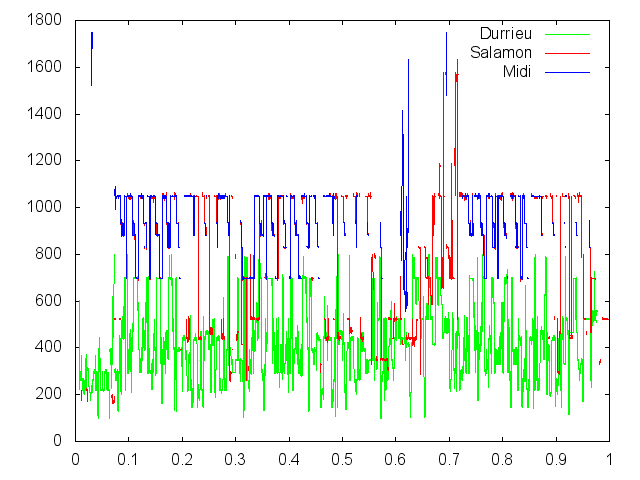
\includegraphics[width=0.7\textwidth]{Figures/Johnny}
\caption{Pitch contours of the ground truth (blue), Durrieu (green) and Salamon (red) for ``Johnny B. Goode'' by Chuck Berry.}
\label{fig:jonny}
\end{figure}


\subsection{Performance}

Although in scientific environment not so important, in case of implementing a game, one of the most important criterion in choosing tools is their speed. We cannot imagine any successful game forcing their users to wait long hours between choosing a music track and being able to play the generated song. The user simply cannot be expected to plan a few hours ahead when and what song they will feel like playing. That is why, apart from investigation of the accuracy of the candidate algorithms, we have to take into account their speed. We present the times it took to generate main melody estimated by each of the algorithms for every song in Table \ref{table:melodytiming}. As we can see, Salamon analyses the songs incomparably faster than Durrieu. In addition to this, it achieves this with higher pitch prediction rate.


\vspace{20pt}

\begin{table}
\begin{center}
\begin{tabular} {| c | c | c | c |} \hline
Title 							& Length 		& Durrieu  						& Salamon  	\\ \hline \hline
Imagine						& 3m 12s		&	4h 5m 53s 570ms 		& 26s 422ms		\\	\hline
Johnny B. Goode		& 2m 20s		&	3h 2m 14s 760ms		& 29s 932ms		\\ 	\hline
Like a Rolling Stone	& 1m 32s		&	1h 59m 52s 630ms		& 9s 193ms		\\ 	\hline
Respect						& 2m 35s		&	3h 23m 38s 610ms		& 12s 597ms		\\ 	\hline
Satisfaction				& 3m 43s		& 	4h 47m 16s 330ms		& 15s 65ms		\\	\hline
\end{tabular}
\caption{Table showing the recall and false alarm for each of the algorithms when analysing against ground truth files.}
\label{table:melodytiming}
\end{center}
\end{table}

\vspace{10pt}


\subsection{Postprocessing}

\begin{figure}[b]     
        \centering
        \begin{subfigure}[b]{0.48\textwidth}
                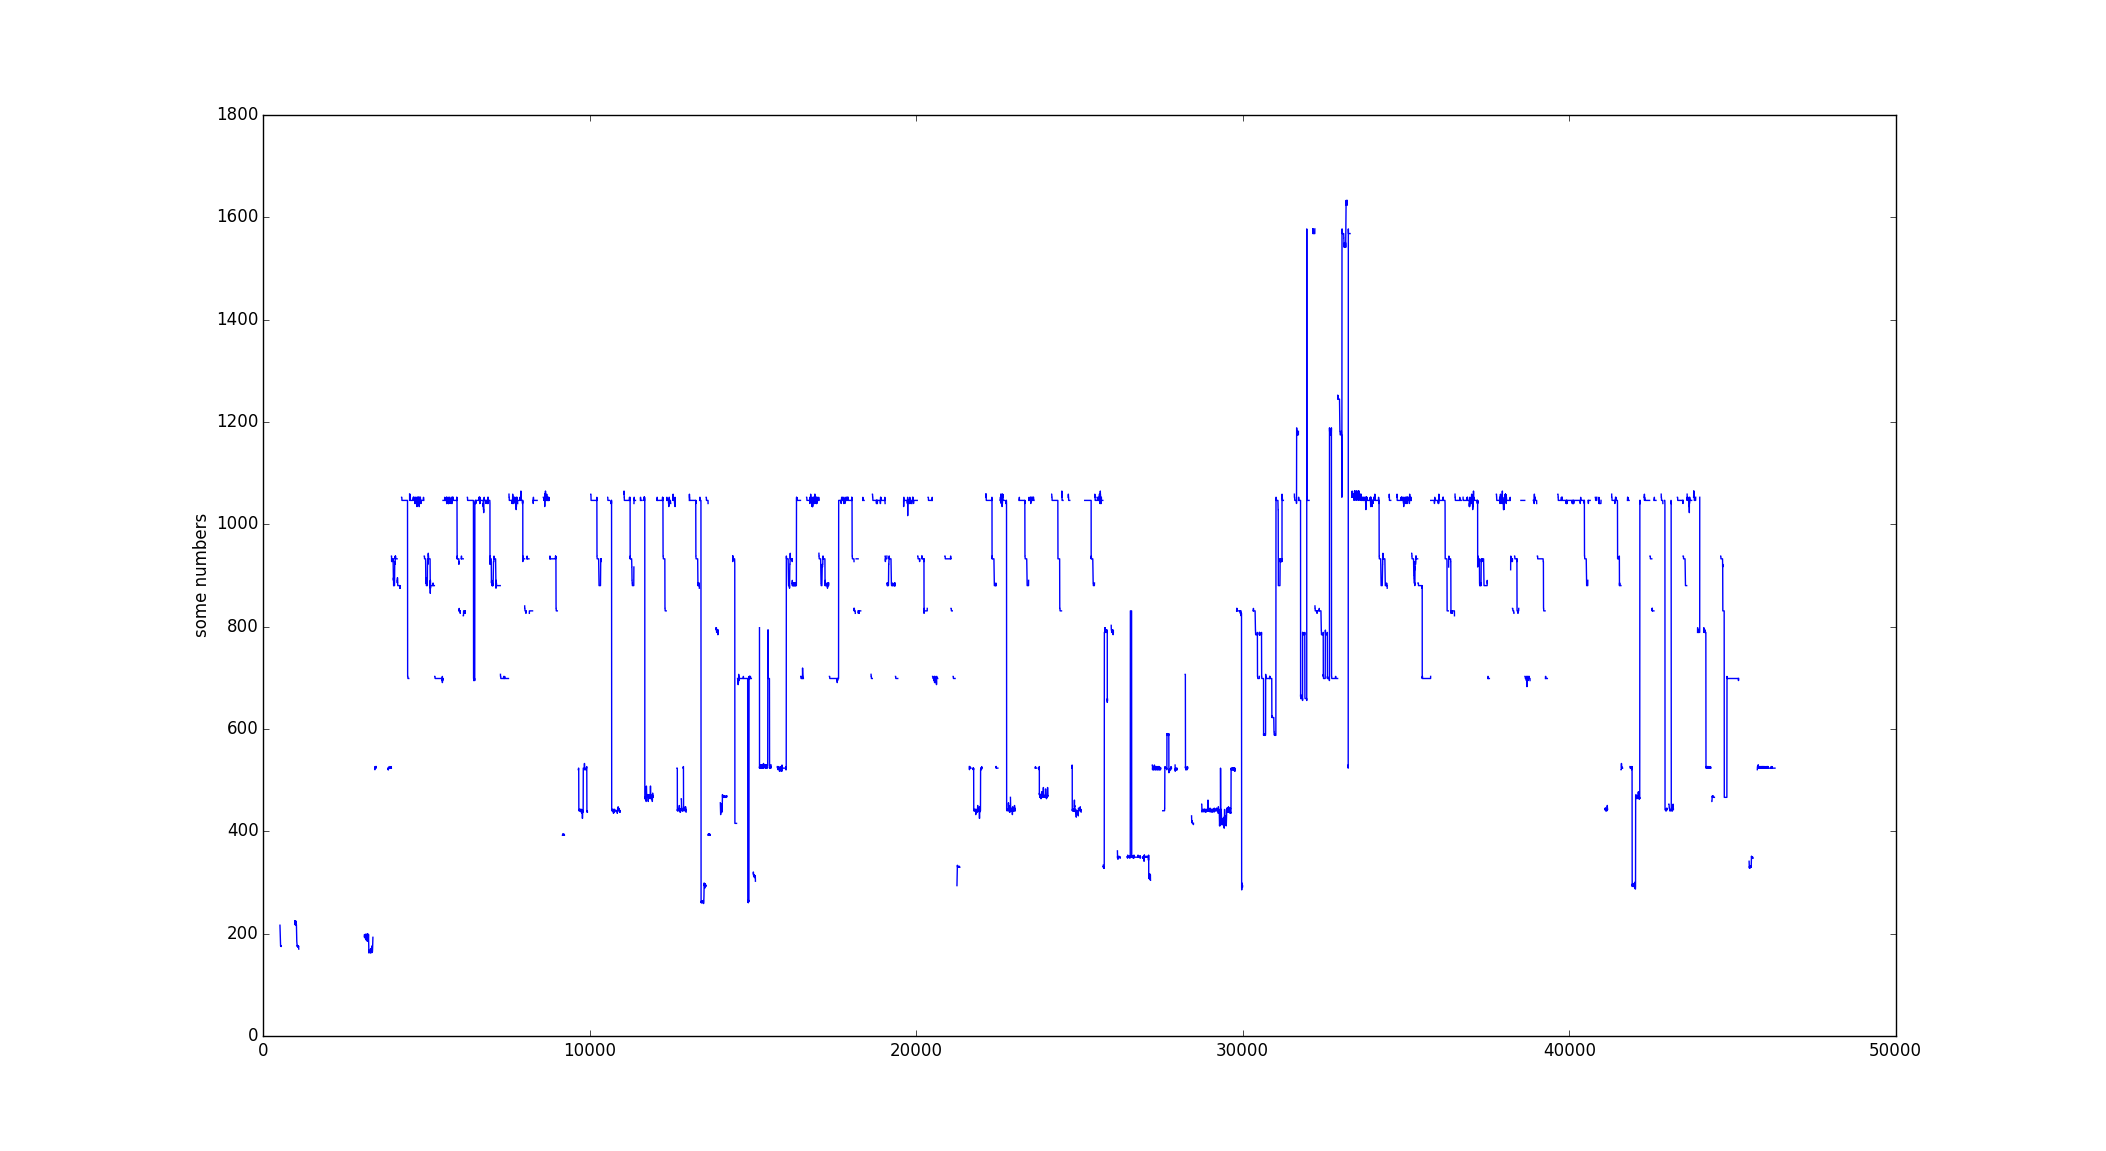
\includegraphics[width=\textwidth]{Figures/input_simple}
                \vspace{20pt}
        \end{subfigure}
        \begin{subfigure}[b]{0.48\textwidth}
                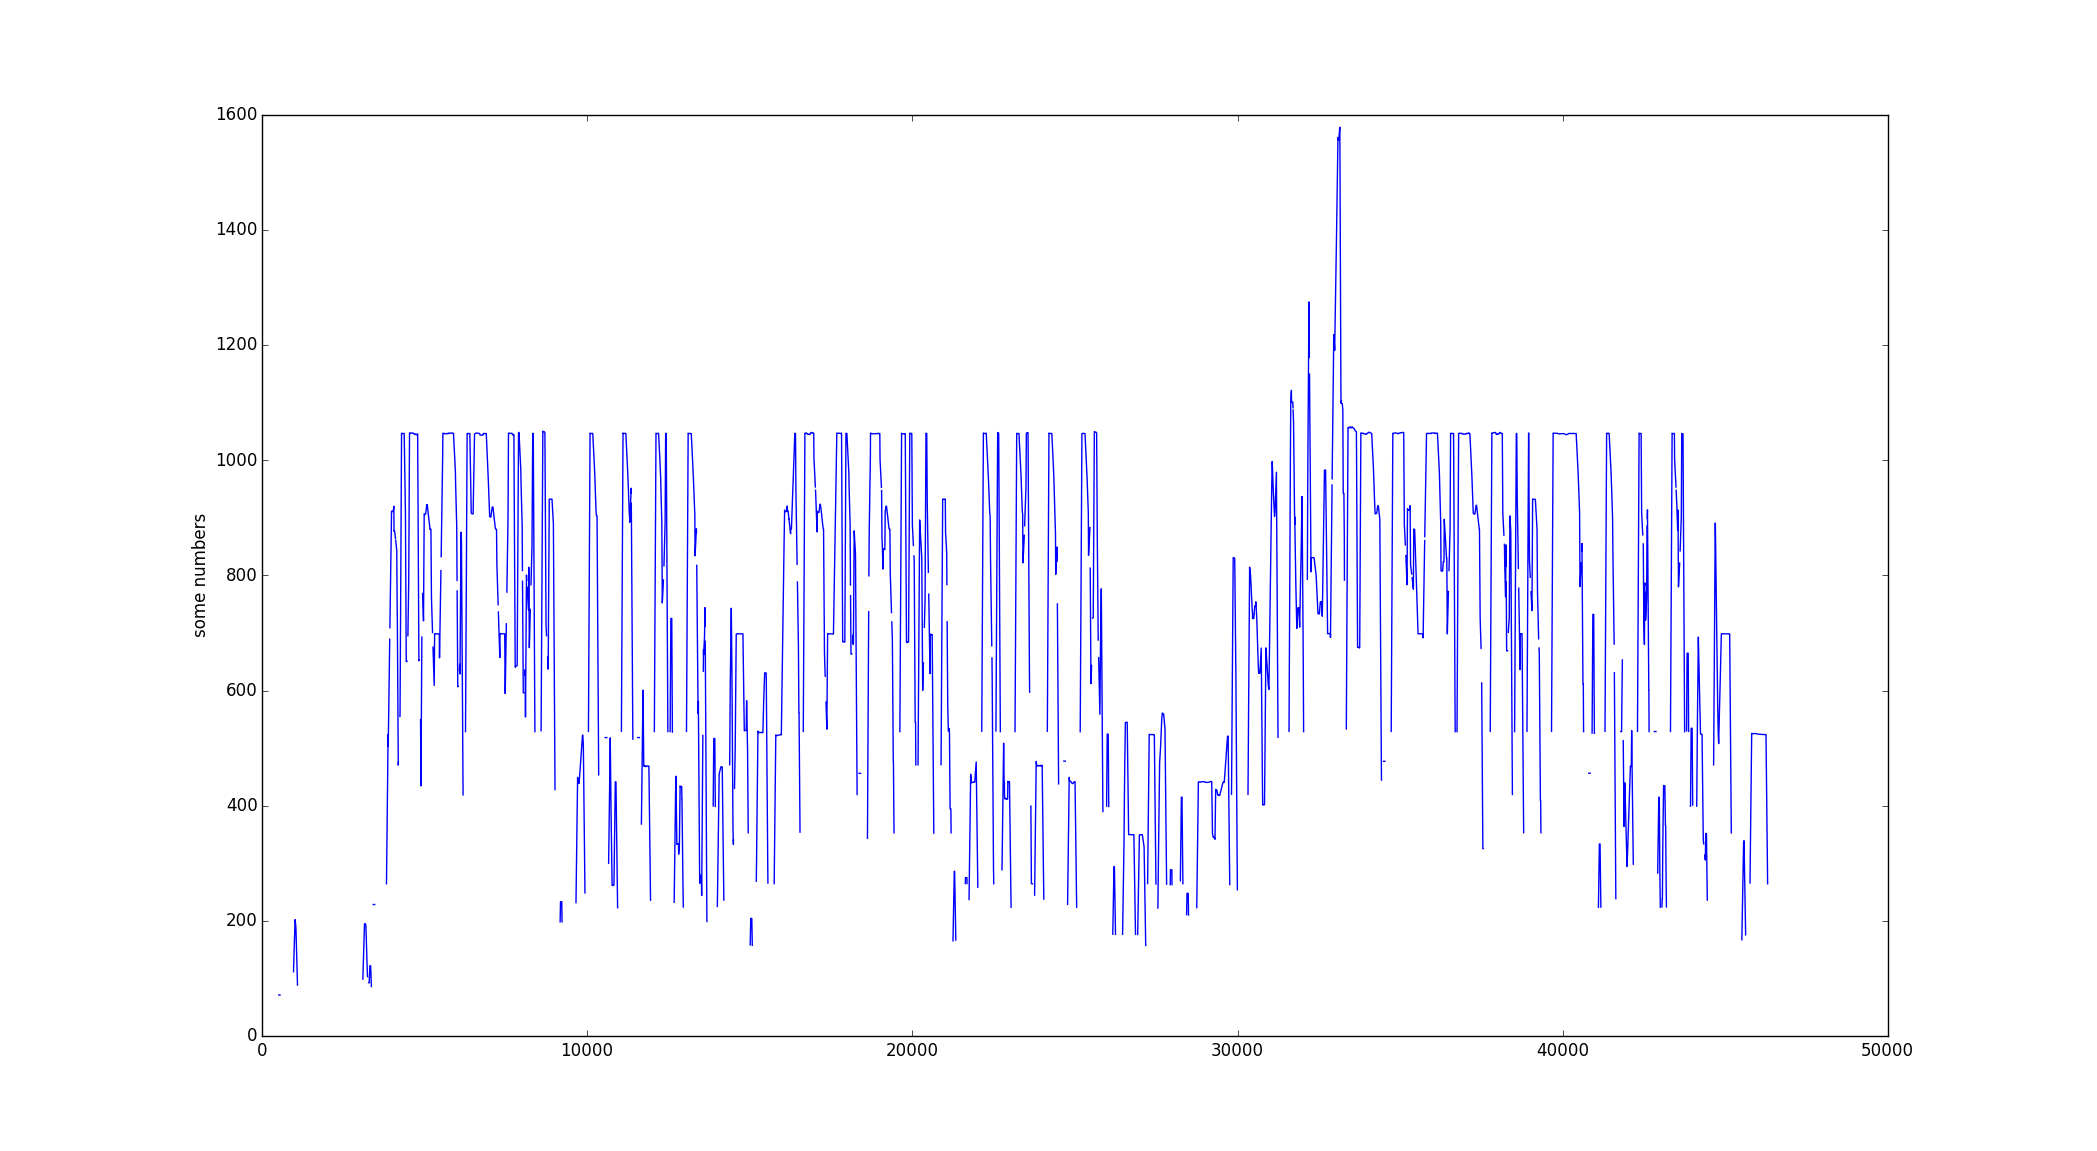
\includegraphics[width=\textwidth]{Figures/rect_101}
                \vspace{20pt}
        \end{subfigure}
    \caption{The pitch contours of the input (left) and created from smoothing the estimated main melody of ``Johnny B. Goode'' by Chuck Berry with additional introduction of false positives (left) and not (right), using the rectangular smooth with $m=101$ (right).}
	\label{fig:rectangular}
\end{figure}

Once we have computed the pitch estimates, we need to post process them to make them more suitable for our application -- we would like to smooth out the pitch contours to avoid sudden spikes. In addition to this, it would be beneficial to be able to control the extent of the smoothing to allow variation in difficulty of the playable song that is going to be generated out of it. 

\begin{figure}[b]
        \centering
        \begin{subfigure}[b]{0.48\textwidth}
                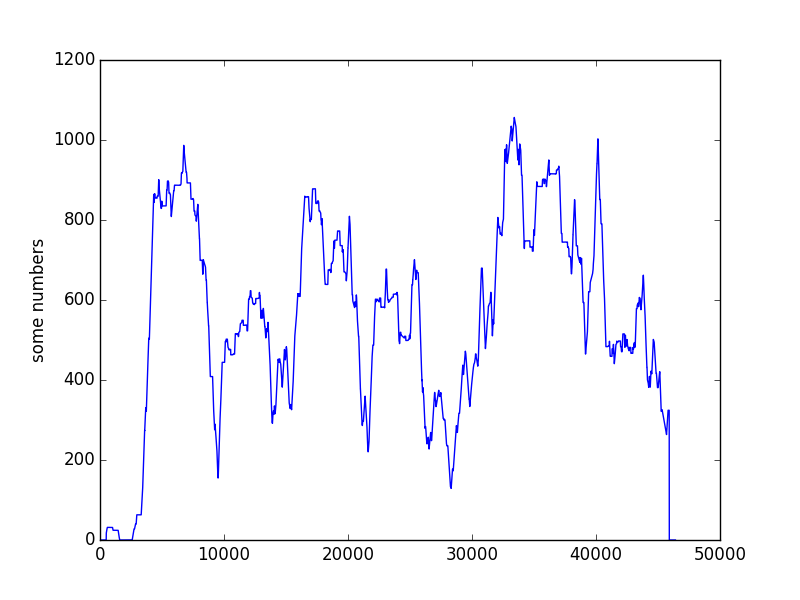
\includegraphics[width=\textwidth]{Figures/smoothing_1001_false}
                \vspace{20pt}
        \end{subfigure}
        \begin{subfigure}[b]{0.48\textwidth}
                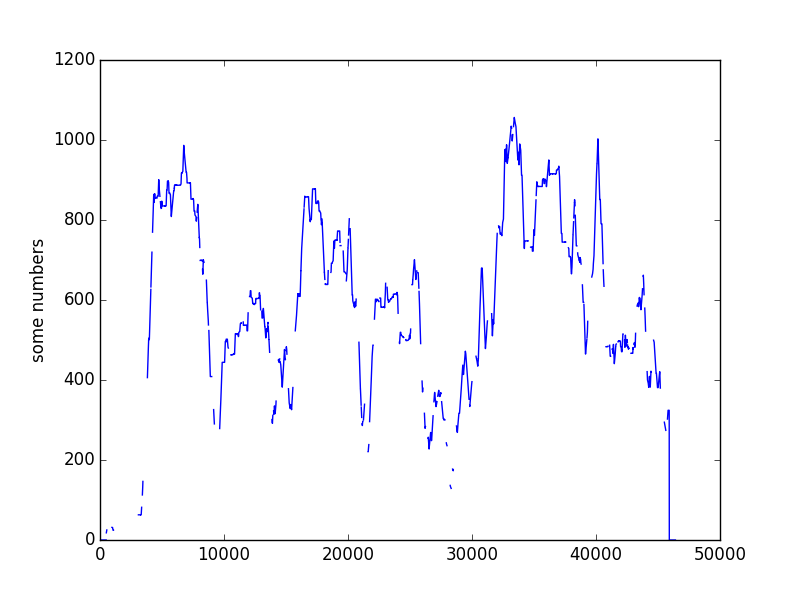
\includegraphics[width=\textwidth]{Figures/smoothing_1001_true}
                \vspace{20pt}
        \end{subfigure}
    \caption{The pitch contours created from smoothing the estimated main melody of ``Johnny B. Goode'' by Chuck Berry with additional introduction of false positives (left) and not (right), using the rectangular smooth with $m = 1001$.}
	\label{fig:excludezeros}
\end{figure}


Most smoothing algorithms are based on the ``shift and multiply" technique, in which a group of adjacent points in the original data are multiplied point-by-point by a set of numbers (coefficients) that defines the smooth shape. The products are added up to become one point of smoothed data, then the set of coefficients is shifted one point down the original data and the process is repeated. 



\begin{figure}[b]        
        \centering
        \begin{subfigure}[b]{0.8\textwidth}
                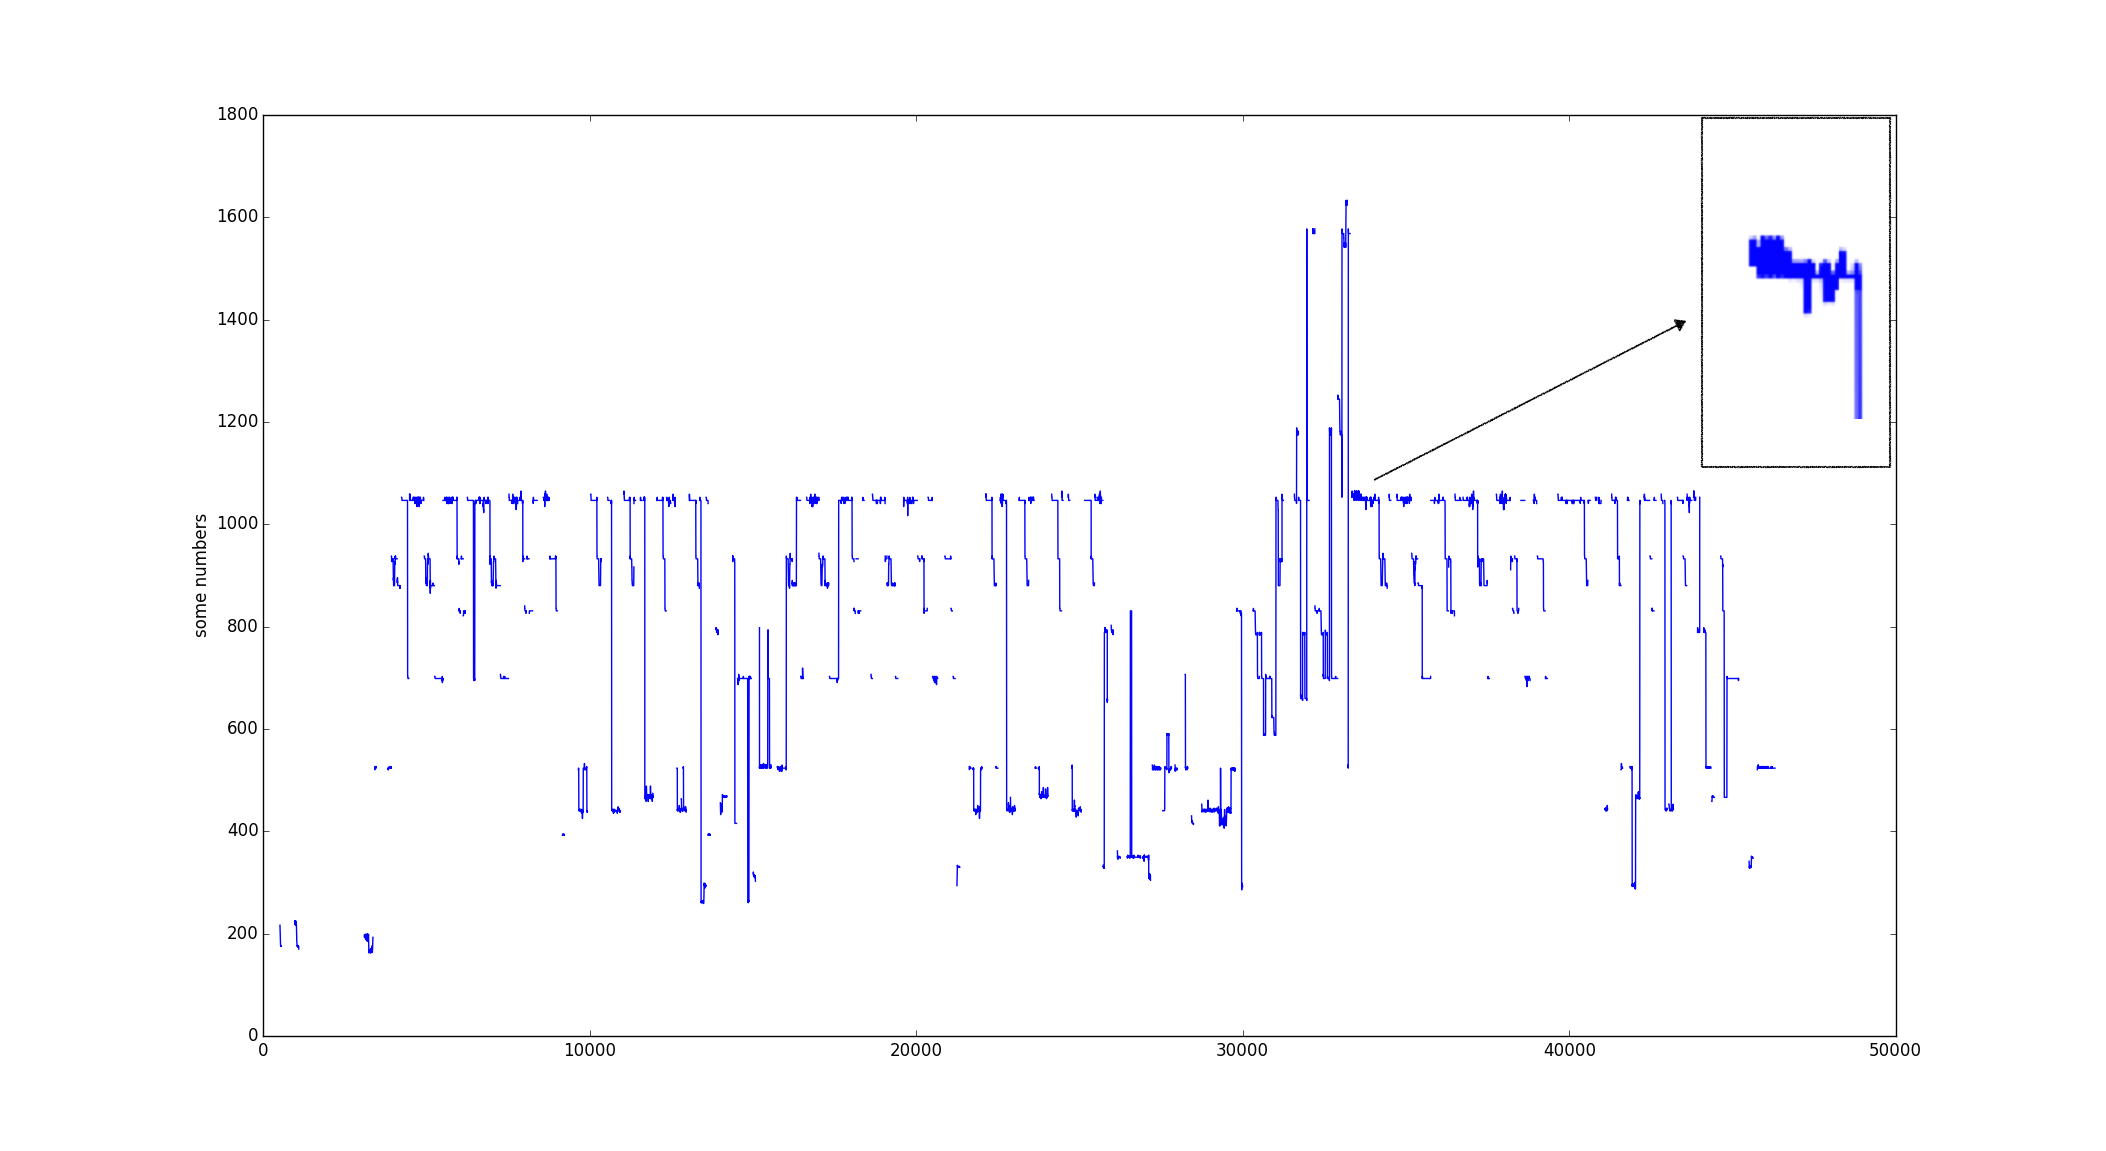
\includegraphics[width=\textwidth]{Figures/input_for_median}
                \vspace{5pt}
        \end{subfigure}
        \begin{subfigure}[b]{0.8\textwidth}
                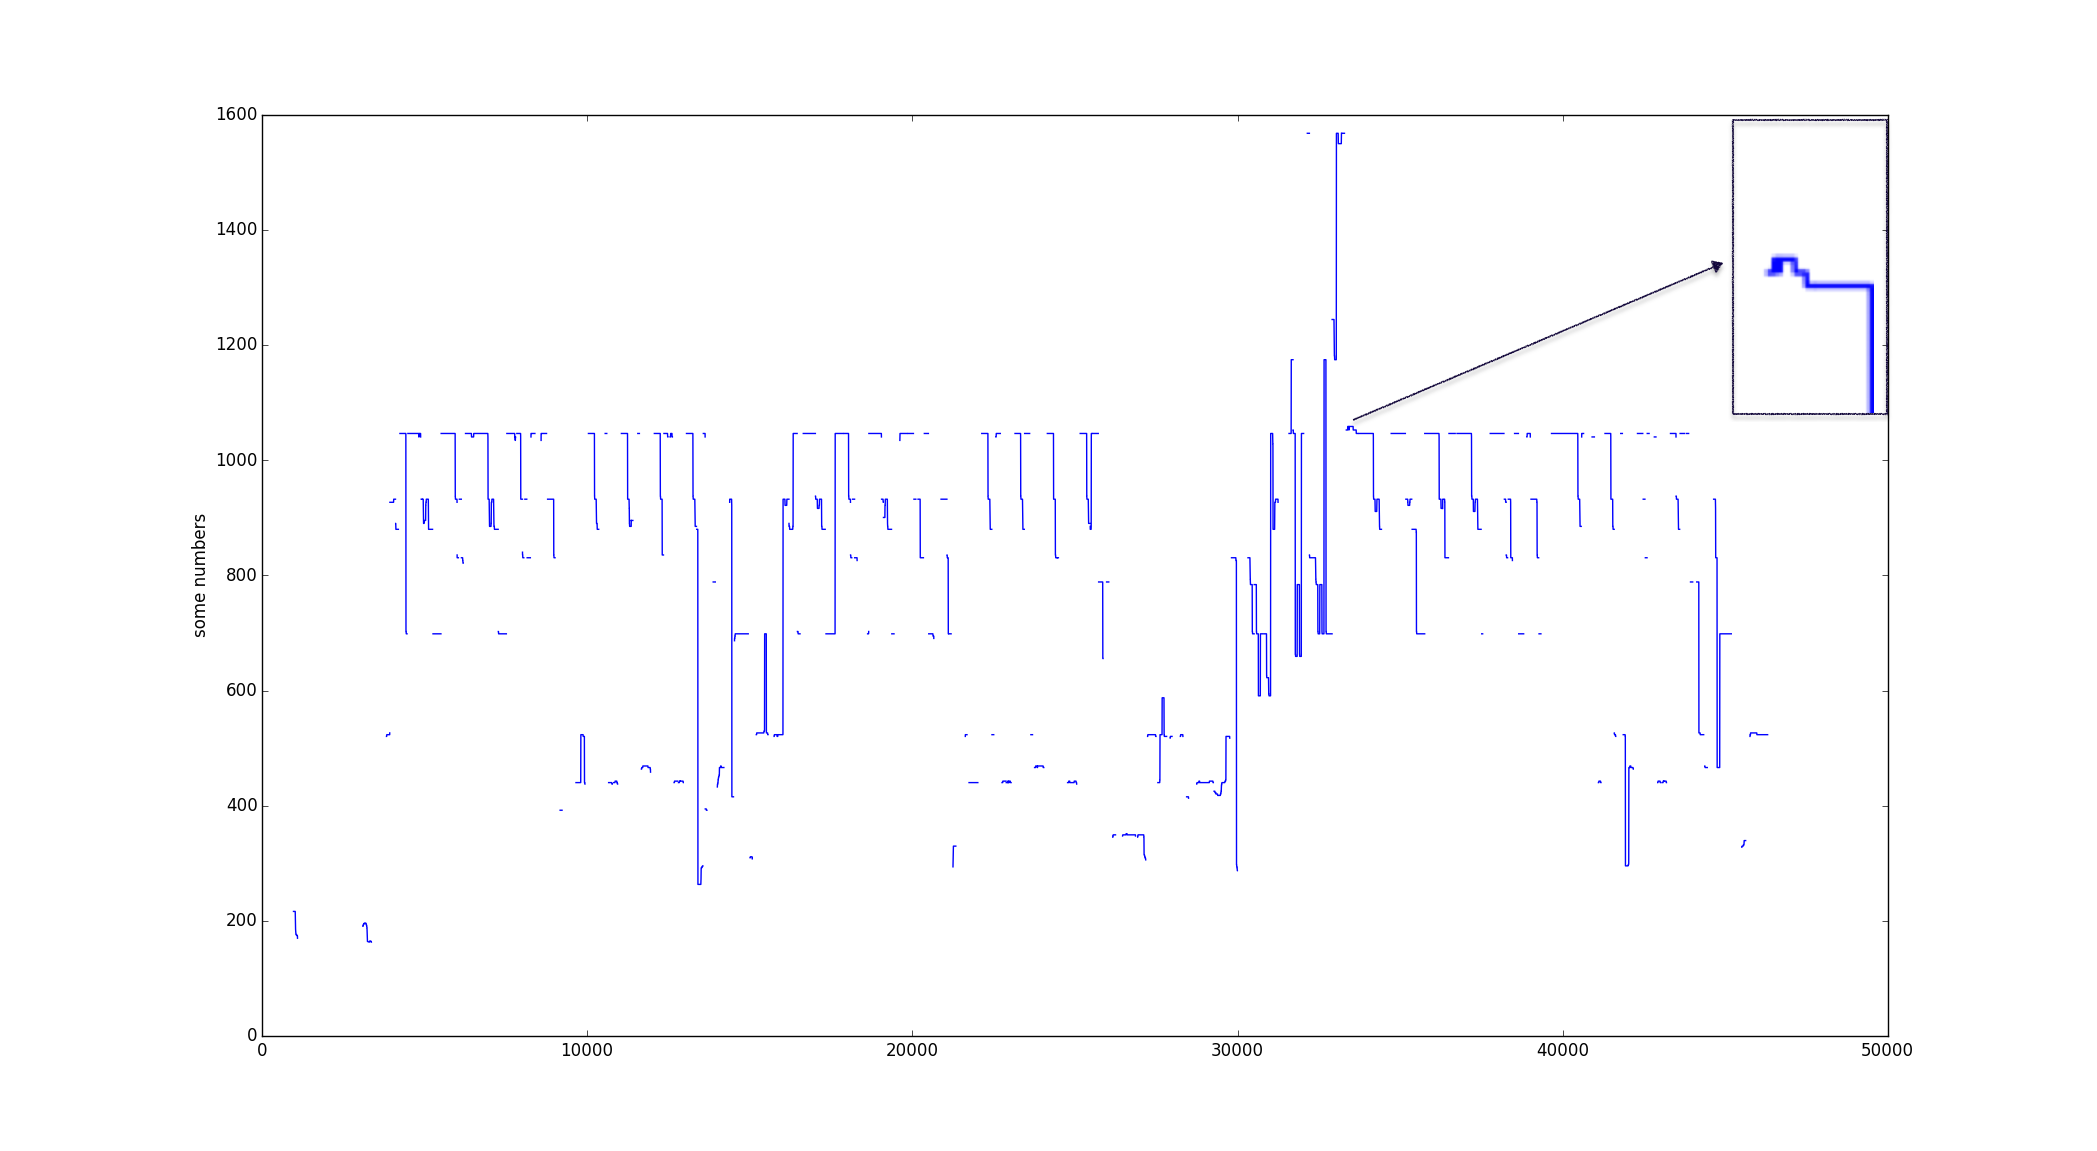
\includegraphics[width=\textwidth]{Figures/median_100_limit}
                \vspace{5pt}
        \end{subfigure}
    \caption{The pitch contours of the input (left) and created by applying the sliding median with window size $w = 100$ to the estimated main melody of ``Johnny B. Goode'' by Chuck Berry.}
	\label{fig:sliding_input}
\end{figure}

The simplest smoothing algorithm is the rectangular or unweighted sliding-average smooth; it simply replaces each point in the signal with the average of $m$ adjacent points, where $m$ is a positive integer called the smooth width. For example, for a 3-point smooth ($m = 3$):
\begin{equation}
	S_{j} = \frac{Y_{j-1} + Y_{j} + Y_{j+1}}{3}
\end{equation}

for $j = 2$ to $n-1$, where $S_{j}$ the $j$th point in the smoothed signal, $Y_{j}$ the $j$th point in the original signal, and n is the total number of points in the signal. 


The results of applying the rectangular sliding average smooth can be seen in Figure \ref{fig:rectangular}. As we can see, even for a window size of 101, which actually is not big when compared to the length of the whole song (in case of this example is over 50,000 frames), the zero values (so the unvoiced frames) drag down the pitch values around them. This is a desirable outcome when dealing with the outliers that were falsely detected as voiced, but introduces more error into correctly detected frames that start the note (so for instance, the first note after a pause).

\begin{figure}
		\vspace{-17pt}
        \centering
 		\begin{subfigure}[b]{\textwidth}
                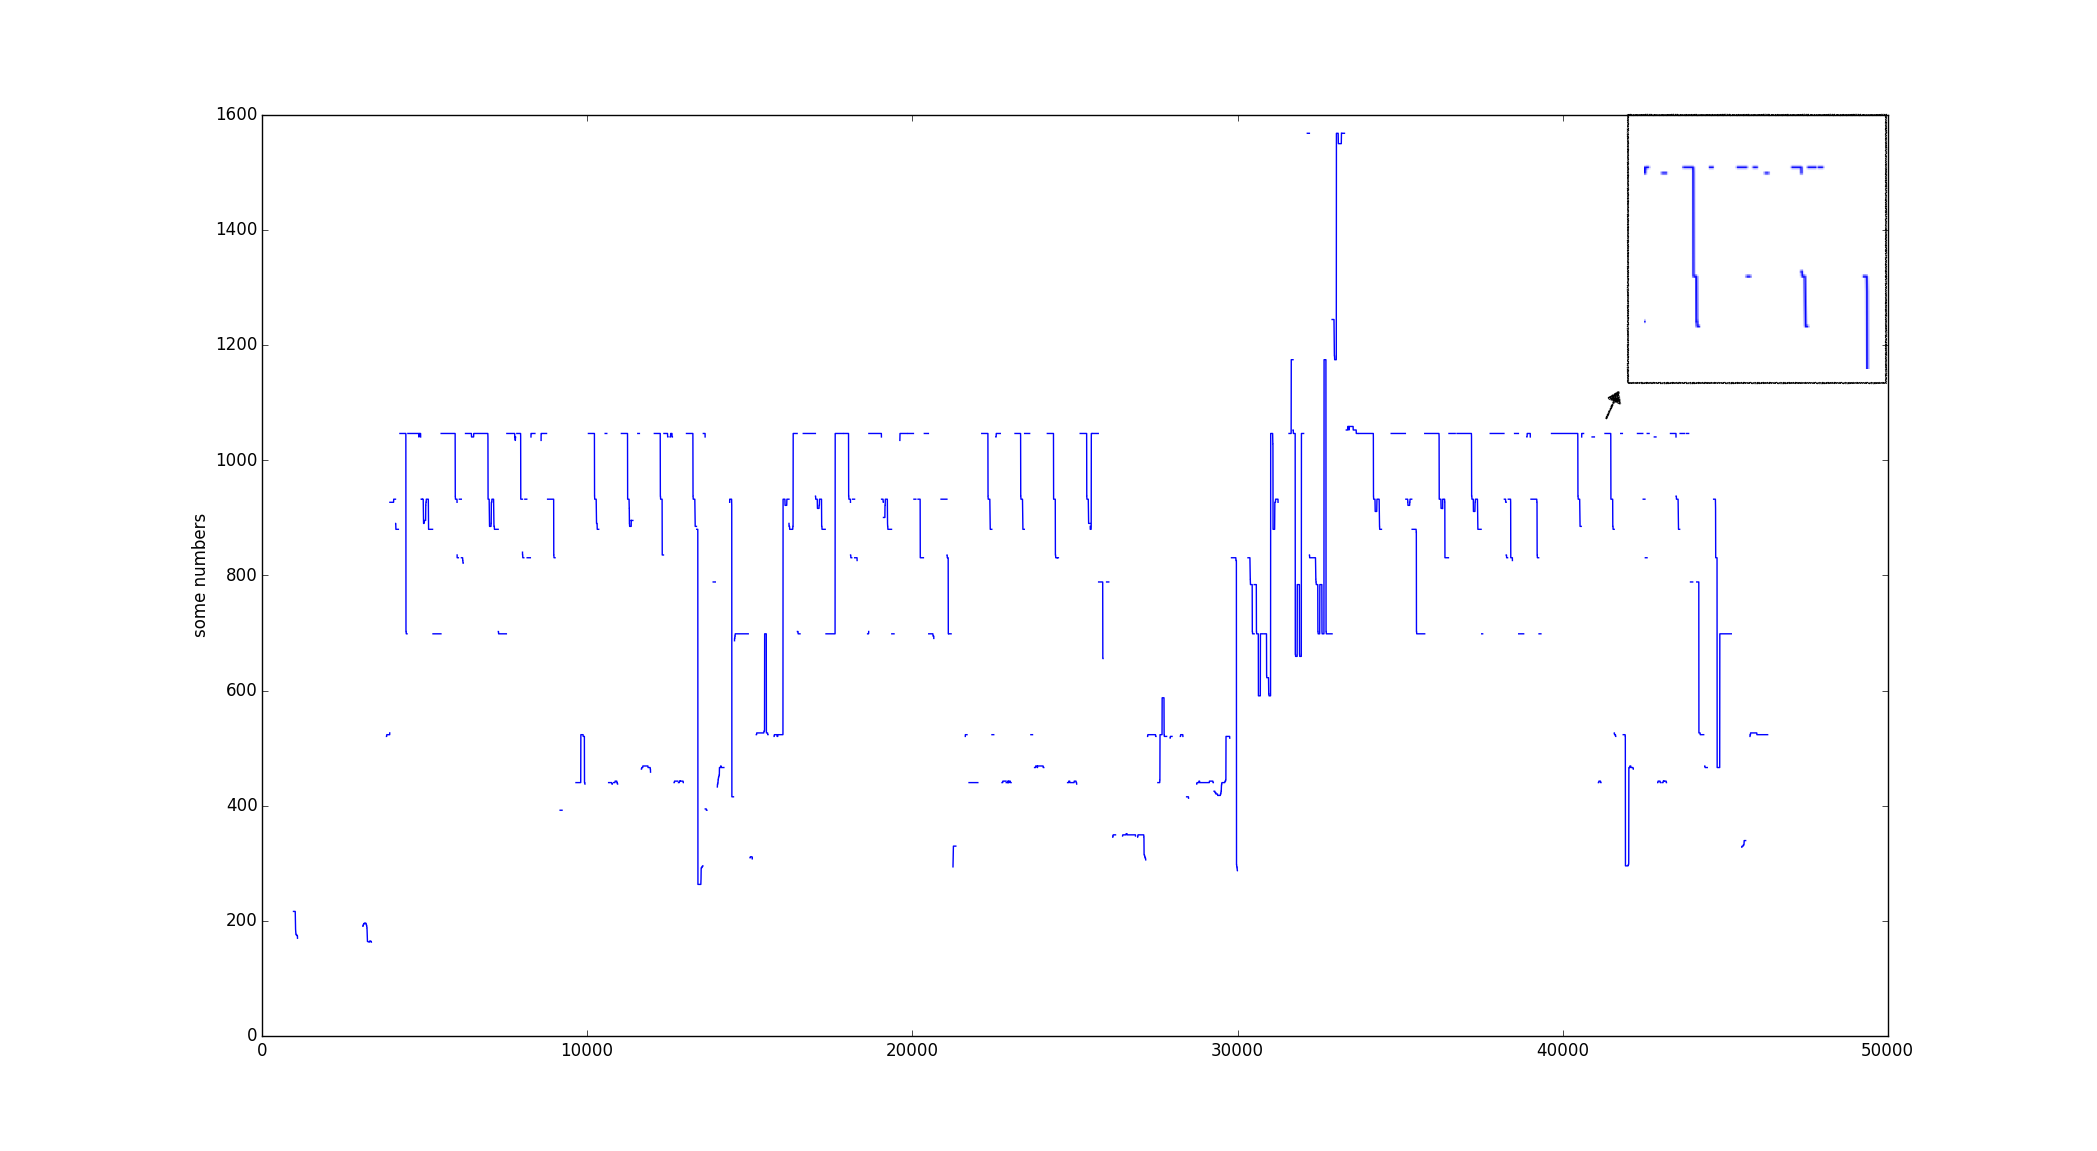
\includegraphics[width=\textwidth]{Figures/sliding_100}
        \end{subfigure}
        \begin{subfigure}[b]{\textwidth}
                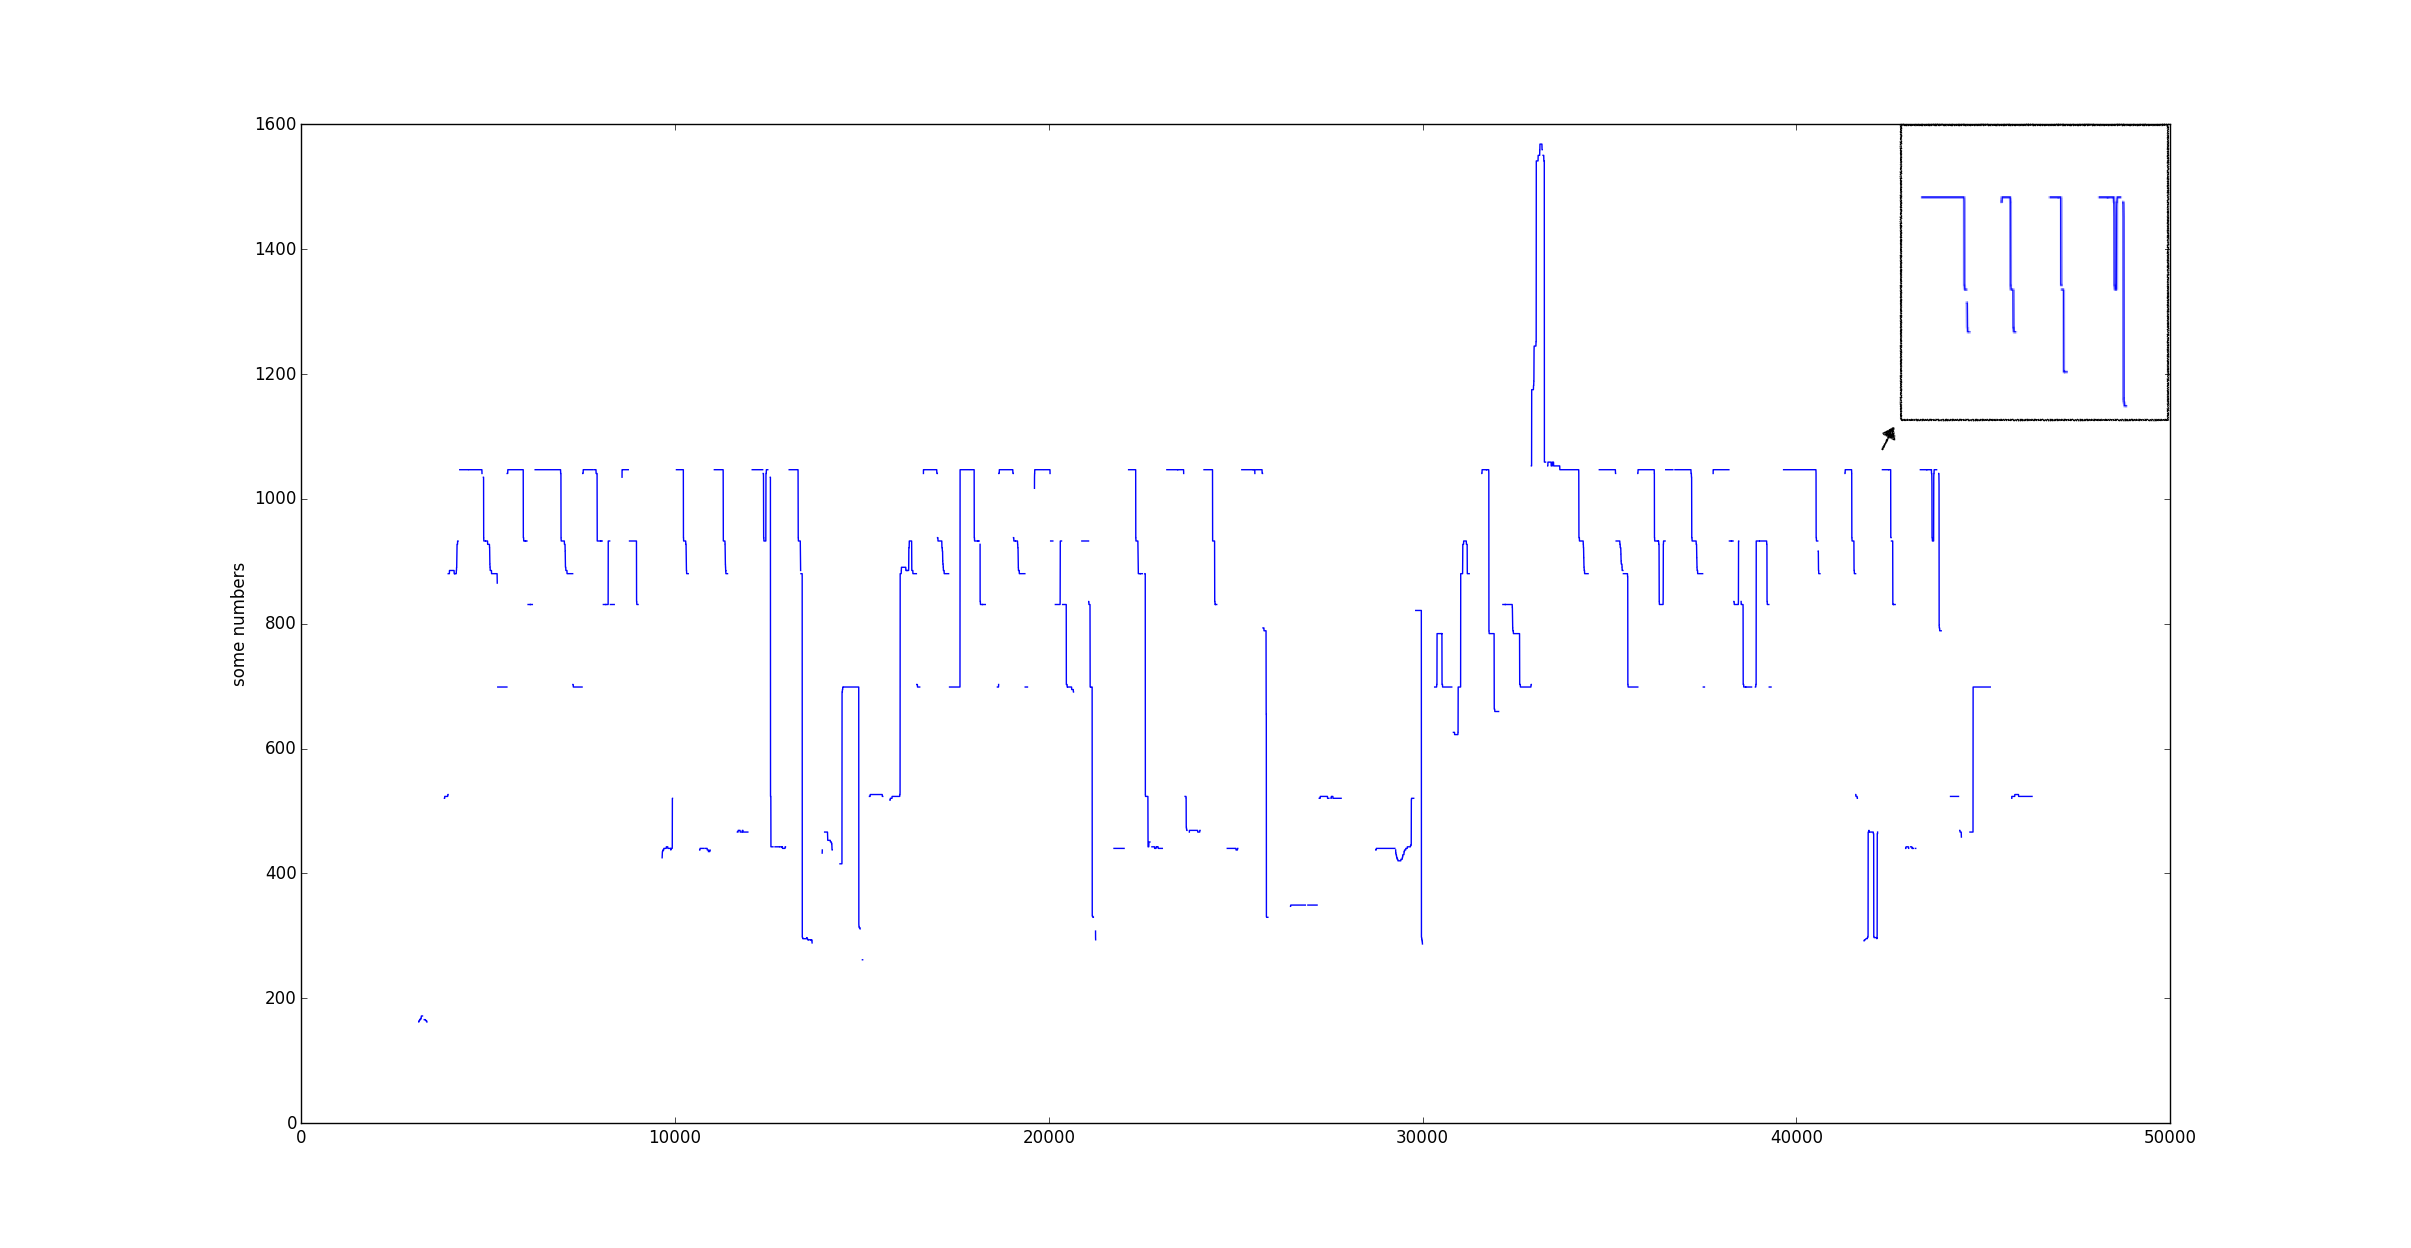
\includegraphics[width=\textwidth]{Figures/sliding_300}
        \end{subfigure}
        \begin{subfigure}[b]{\textwidth}
                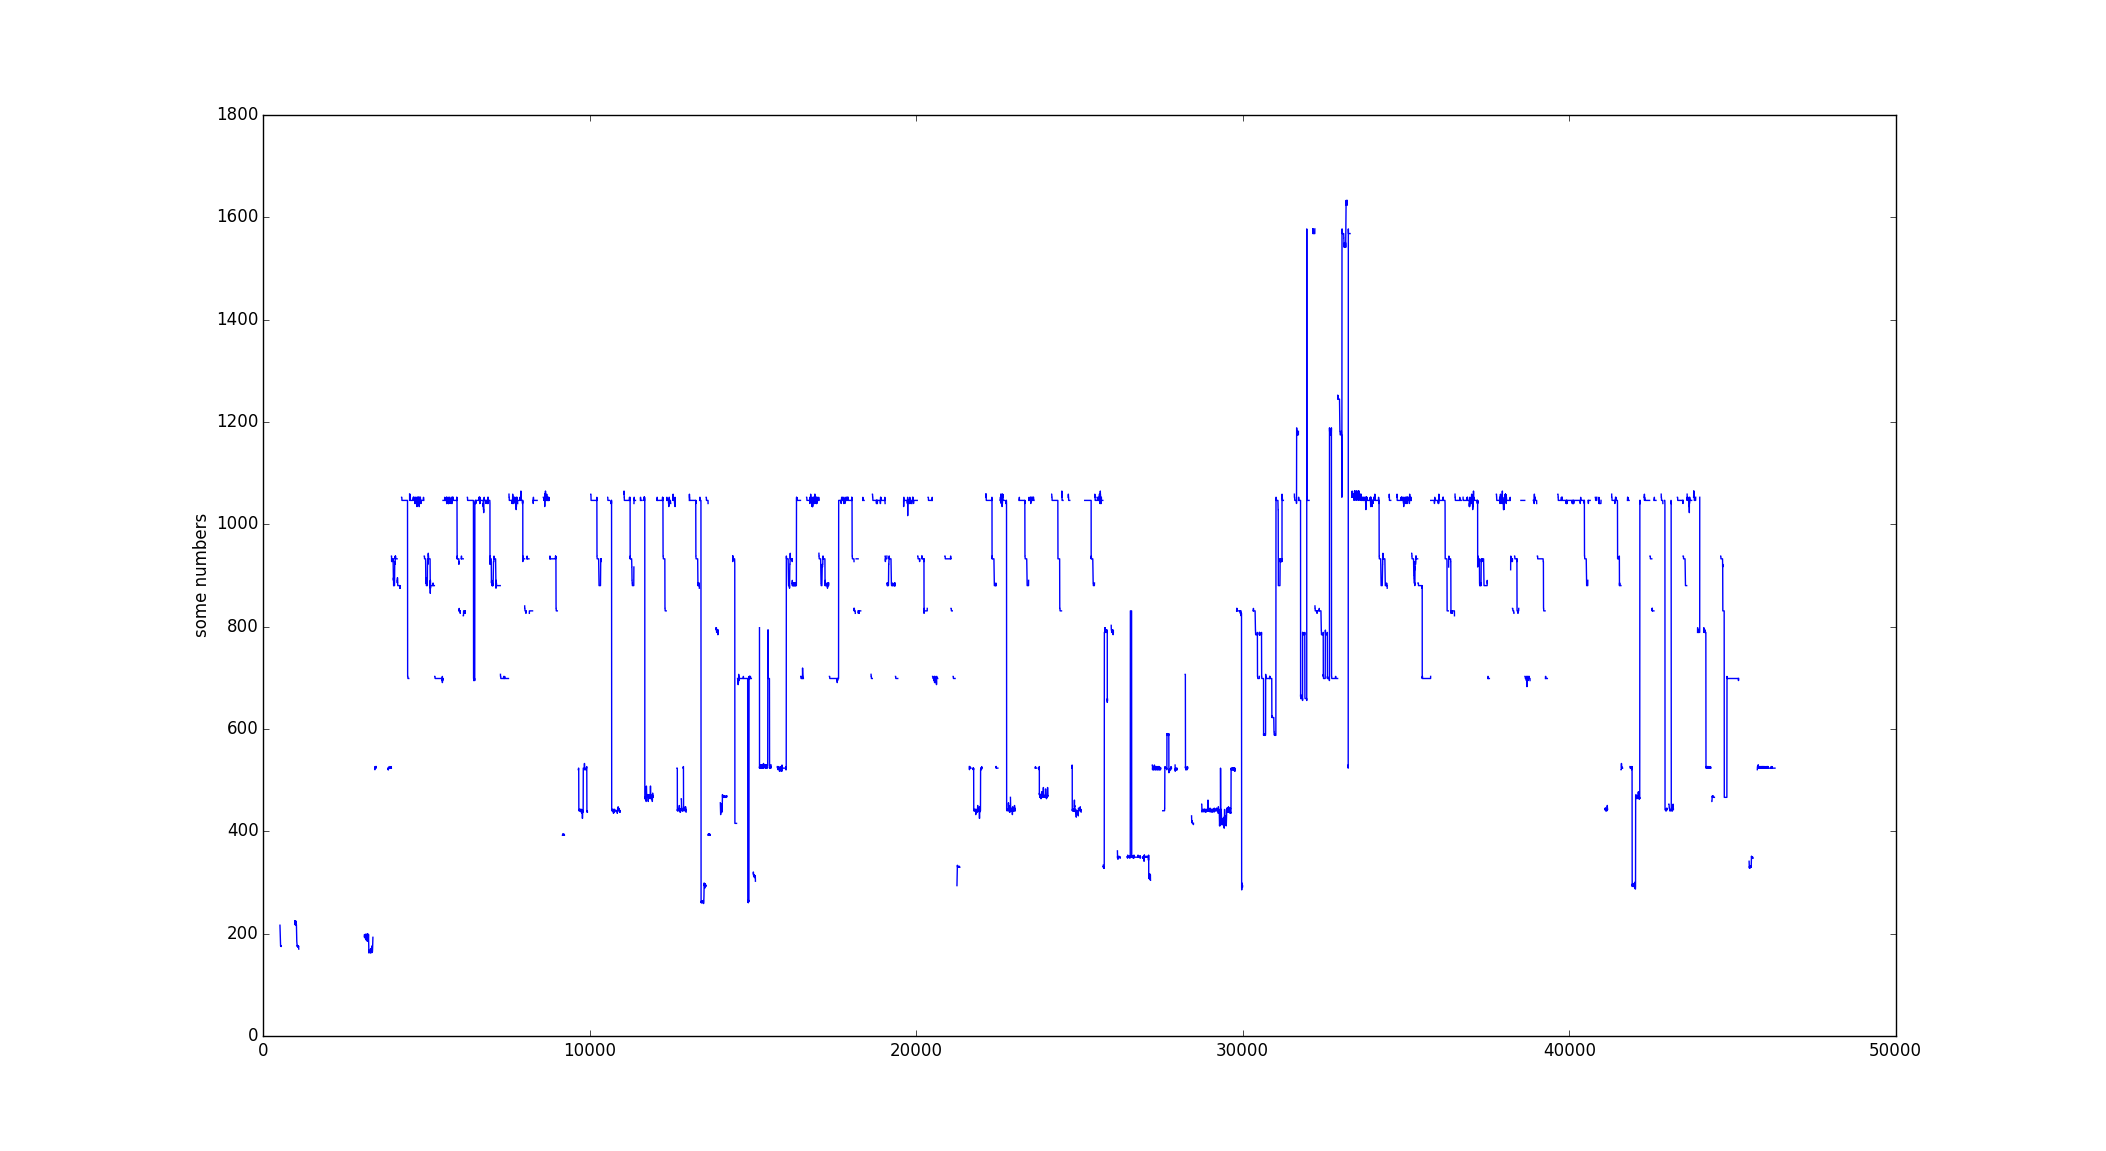
\includegraphics[width=\textwidth]{Figures/input_simple}
        \end{subfigure}
    \caption{The pitch contours created by applying the sliding median with window size $w = 100$ (top), $w = 300$ (middle) and the initial input (bottom).}
	\label{fig:sliding_comp}
\end{figure}

Another solution to the problem is to use the sliding median filter. The main idea behind it is to run through the signal entry by entry, replacing each of them with the median of neighboring entries. The pattern of neighbors is called the ``window", which slides, entry by entry, over the entire signal. 

For 1D signals, the most obvious window is just the first few preceding and following entries, whereas for 2D (or higher-dimensional) signals such as images, more complex window patterns are possible (such as ``box" or ``cross" patterns). Note that if the window has an odd number of entries, then the median is simple to define: it is just the middle value after all the entries in the window are sorted numerically. For an even number of entries, there is more than one possible median.

The impact of applying the sliding median of size 100 on the estimated pitches can be seen in Figure \ref{fig:sliding_input}. On the other hand, comparison of the results for the different window sizes can be seen in Figure \ref{fig:sliding_comp}. As we can see, applying a bigger window size smooths the contours even more. Although this way the main melody loses some of its elements, like when the voice is quickly vibrating, it can prove useful when generating simpler songs to play, as the changes in the pitch will be less frequent, making the melody less complex and hence, less interaction will be required from the user. 

An important thing in our application is that we do want to preserve our zero values in our smoothed pitch coutours. If we fail to do so, we introduce additional false positives in our voicing detection. The visualisation of the problem can be seen in Figure \ref{fig:excludezeros}.

\vspace{20pt}


\section{Structure Retrieval}

Understanding the structure of music (i.e. localisation of different parts such as intro, verse, chorus, bridge, and outro) is important as it allows us to divide a song into semantically meaningful segments, within which musical characteristics are relatively consistent.

\vspace{10pt}

\subsection{Feature Choice}

To implement a system capable of unsupervised structure recognition, we needed to provide it with some data. We investigated two possible values - \textit{Mel-frequency cepstral coefficients} and \textit{harmonic pitch class profile}.

Harmonic pitch class profiles (HPCP) is a vector of features extracted from an audio signal, based on the Pitch Class Profile descriptor. It is an enhanced pitch distribution feature which is described by a sequence of chroma - feature vectors describing tonality measuring the relative intensity of each of the 12 pitch classes of the equal-tempered scale within an analysis frame. 

HPCP features can be found and used to estimate the key of a piece, to measure similarity between two musical pieces and to classify music in terms of composer, genre or mood. The process is related to time-frequency analysis. In general, chroma features are robust to noise, for example an ambient noise or percussive sounds, independent of timbre and instrumentation and independent of loudness and dynamics.

The General HPCP feature extraction procedure is summarised as follows:
\begin{itemize}
\item Input musical signal.
\item Do spectral analysis to obtain the frequency components of the music signal.
\item Use Fourier transform to convert the signal into a spectrogram.
\item Do frequency filtering. A frequency range of between 100 and 5000 Hz is used.
\item Do peak detection. Only the local maximum values of the spectrum are considered.
\item Do reference frequency computation procedure. Estimate the deviation with respect to 440 Hz.
\item Do Pitch class mapping with respect to the estimated reference frequency. This is a procedure for determining the pitch class value from frequency values. A weighting scheme with cosine function is used. It considers the presence of harmonic frequencies (harmonic summation procedure), taking account a total of 8 harmonics for each frequency. In order to map the value on a one-third of a semitone, the size of the pitch class distribution vectors has to be equal to 36.
\item Normalise the feature frame by frame dividing through the maximum value to eliminate dependency on global loudness.
\end{itemize}

An alternative to using HPCPs as the features to base the algorithm on is \textit{Mel-frequency cepstral coefficients}.

The term ``cepstrum'' refers to the result of taking the Inverse Fourier transform (IFT) of the logarithm of the estimated spectrum of a signal. It can be viewed as information about rate of change in the different spectrum bands.

The mel-frequency cepstrum (MFC) is a representation of the short-term power spectrum of a sound, based on a linear cosine transform of a log power spectrum on a nonlinear mel scale of frequency. 

\textit{Mel-frequency cepstral coefficients} (MFCCs) are coefficients that collectively make up an MFC. They are increasingly finding uses in music information retrieval applications such as genre classification, audio similarity measures, etc.

MFCCs are perceptually based spectral features originally designed for speech processing applications. Similarly to the pitch decomposition, the frequency bands are positioned logarithmically on the so-called mel scale, which approximates the response of the human auditory system. In the music context, MFCCs have turned out to be useful in capturing timbral characteristics.

MFCCs are derived from a type of cepstral representation of the audio clip. The mel-frequency cepstrum differs from cepstrum by having its frequency bands equally spaced on the mel scale, which approximates the human auditory system's response more closely than the linearly-spaced frequency bands used in the normal cepstrum. This frequency warping can allow for better representation of sound, for example, in audio compression \cite{mfcc}

MFCCs are commonly derived as follows:
\begin{itemize}
\item Take the Fourier transform of a signal.
\item Map the powers of the spectrum obtained above onto the mel scale, using triangular overlapping windows.
\item Take the logs of the powers at each of the mel frequencies.
\item Take the discrete cosine transform of the list of mel log powers, as if it were a signal.
\item The MFCCs are the amplitudes of the resulting spectrum.
\end{itemize}

\vspace{10pt}

\subsection{Feature Preparation}

In this section, we will describe the process of preparation of the features for improving the performance of the algorithm. For simplicity and clarity, when talking about the features, we will first focus on analysis based on HPCPs, followed by one on MFCCs.
We decided to investigate both possibilities as they present the music track from completely different perspective. For example, the HPCP chroma might fail to distinguish vocal and instrumental parts if the underlying harmonic patterns are exactly the same. On the other hand, when working with MFCCs we expected the opposite behaviour - good performance on parts that are different in terms of timbre.

\subsubsection*{Harmonic Pitch Class Profiles}

\begin{figure}
        \centering
        \begin{subfigure}{0.47\textwidth}
                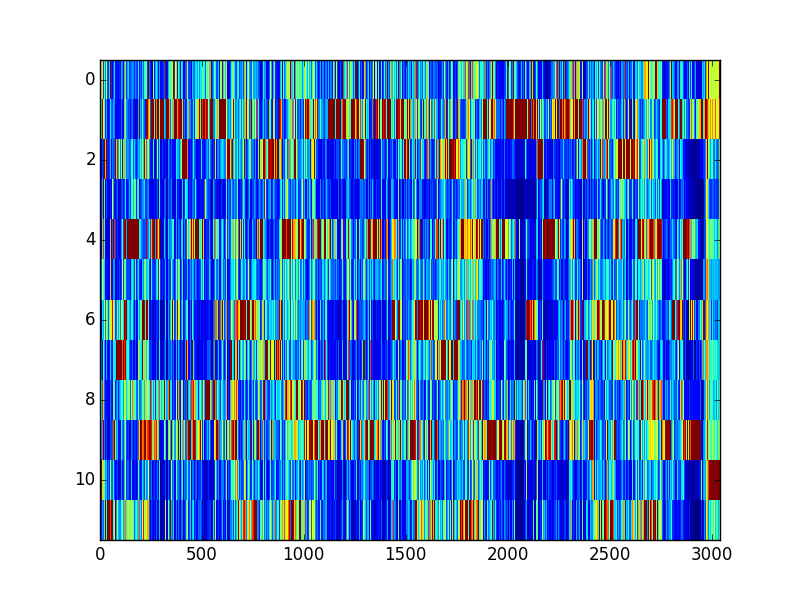
\includegraphics[width=\textwidth]{Figures/hpcp_unsynched_chroma}
                \caption{Example of a chromagram without any further enhancement. }
                \label{fig:unchroma}
        \end{subfigure}
        \begin{subfigure}{0.47\textwidth}
                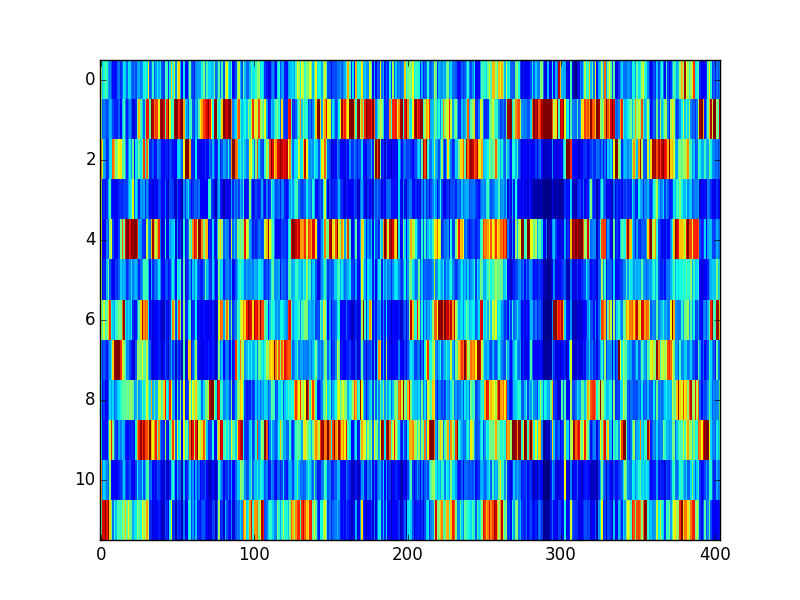
\includegraphics[width=\textwidth]{Figures/hpcp_synched_chroma}
                \caption{Example of a chromagram after beat-synchronisation.}
                \label{fig:synchroma}
        \end{subfigure}
          \caption{Harmonic pitch class profiles chroma features calculated for a song by The Beatles- ``Help!''.}
        \label{fig:chromacomparison}
\end{figure}

A series of transformations were applied to the data in order to distinguish the different parts of a song more efficiently with preserving the accuracy.

\begin{figure}[t]
        \centering
        \begin{subfigure}[b]{0.47\textwidth}
                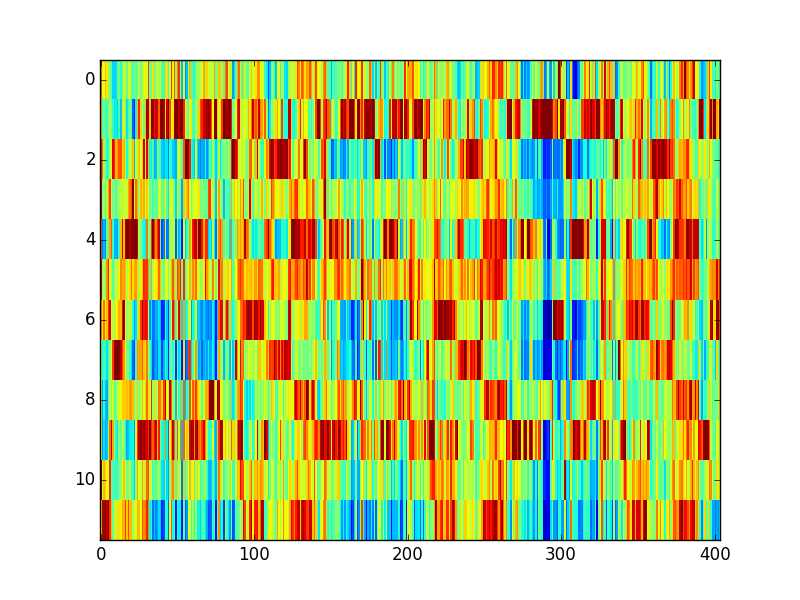
\includegraphics[width=\textwidth]{Figures/hpcp_synched_log_chroma}
                \caption{Chroma feature after applying log normalisation.}
                \label{fig:logchroma}
        \end{subfigure}%
        \begin{subfigure}[b]{0.47\textwidth}
                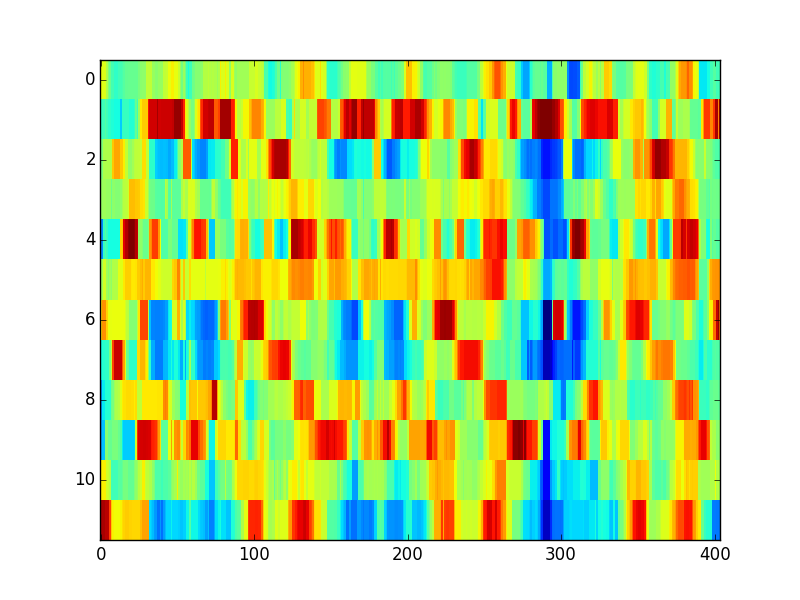
\includegraphics[width=\textwidth]{Figures/hpcp_synched_median_chroma}
                \caption{Chroma feature after applying sliding median filter of size $h=9$.}
                \label{fig:slidingchroma}
        \end{subfigure}
          \caption{Beat-synchronised chroma created for song ``Help!'' by The Beatles with applied enhancements.}
        \label{fig:chromaenhance}
\end{figure}


First, we needed to we synchronise our data with the beats detected in the musical track. This process allowed to reduce local variation by summarising frame-wise features that occur between two beats, yielding fewer but longer beat-synchronous frames. The rationale for doing so was that many features, such as chord labels that occur between two consecutive beats tend to be the same. Thanks to focusing on the values of the features on a per-beat basis, we managed to largely normalise variations in tempo. However, the main advantage of applying the beat-synchronisation was that we managed to reduce the amount of data to analyse, and hence, the size of the matrix, we were operating on.

\begin{figure}[b]
        \centering
        \begin{subfigure}[b]{0.47\textwidth}
                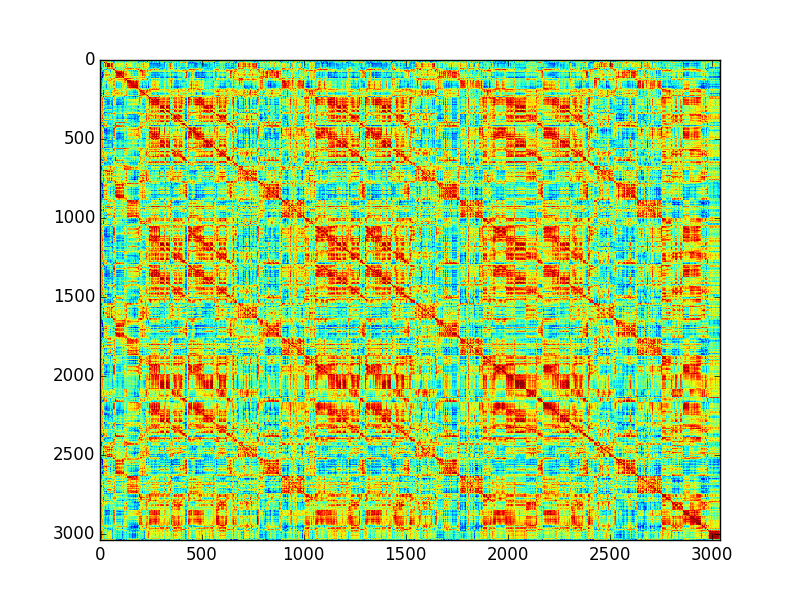
\includegraphics[width=\textwidth]{Figures/hpcp_unsynched_ssm}
                \caption{Self-similarity matrix generated from harmonic pitch class profiles chroma without further enhancement.}
                \label{fig:unSSM}
        \end{subfigure}%
        \begin{subfigure}[b]{0.47\textwidth}
                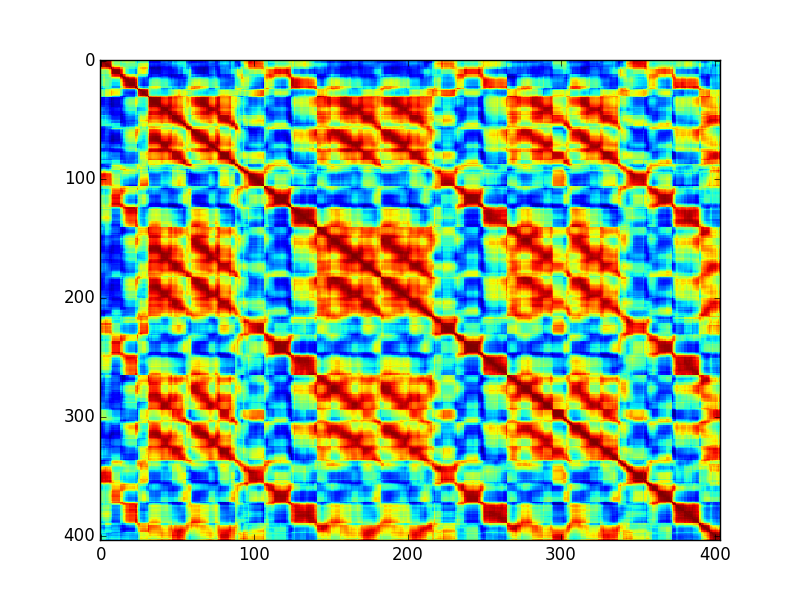
\includegraphics[width=\textwidth]{Figures/log_ssm_synched}
                \caption{Self-similarity matrix generated from beat-synchronised harmonic pitch class profiles chroma.}
                \label{fig:synSSM}
        \end{subfigure}
          \caption{Comparison of SSM generated from unprocessed and enhanced chromas, using correlation distance.}
        \label{fig:ssmcomparison}
\end{figure}

This led us to beat-synchronous chromagrams. A diagram of a chromagram after beat synchronisation can be seen in Figure \ref{fig:synchroma}. As we can see, the size has decreased dramatically, which makes the segmentation process computationally cheaper.

Following the beat-synchronisation, we applied log normalisation to the chroma feature. This allowed us to reduce the effect the outliers from the trend would have and further improve the contrast between the related and unrelated beat frames. The enhancement achieved by applying log normalisation can be seen in Figure \ref{fig:logchroma}.

As the next step, we applied a sliding median filter of size $h$ is run against each of the beat-synchronous and log-normalised chromagram channels. Thanks to the median filter, we could come up with sharper edges than with a regular mean filter. This became really useful in obtaining section boundary precision.

By filtering features across time, we retained the most prominent chromas within the h-size window and removed smaller artefacts, which are irrelevant in our context. The Figure \ref{fig:slidingchroma} presents the chromagram after applying the sliding median filter.

We then proceeded to compute the self-similarity matrix (SSM) of the pre-filtered beat-synchronous chromagram. The SSM is essentially a pairwise comparison of a given set of features using a specific distance measure between the features of the two beat indices i and j. The result of every such comparison is stored in a $N \times N$ symmetric matrix $D$, such that $D(i, j)$ contains said distance. In particular, $D(i, j)$ stores the same value as $D(j, i)$, and for every $i$ $D(i, i)$ is equal to 0.

We investigated the influence of the type of the distance calculated on the SSM produced for the enhanced chroma. In our research we looked into four types of distance: Euclidean, Manhattan, correlation and cosine. Our results are presented in Figure \ref{fig:ssmdistance}. 
As we can see in Figures \ref{fig:euclidean} and \ref{fig:manhattan}, the contrast achieved for SSM produced using Euclidean and Manhattan distances was much weaker. Not only there were fewer blue spots signifying small or no similarity between points, but the amount of points that were significantly similar was also reduced.


\begin{figure}[t]
        \centering
        \begin{subfigure}[b]{0.31\textwidth}
                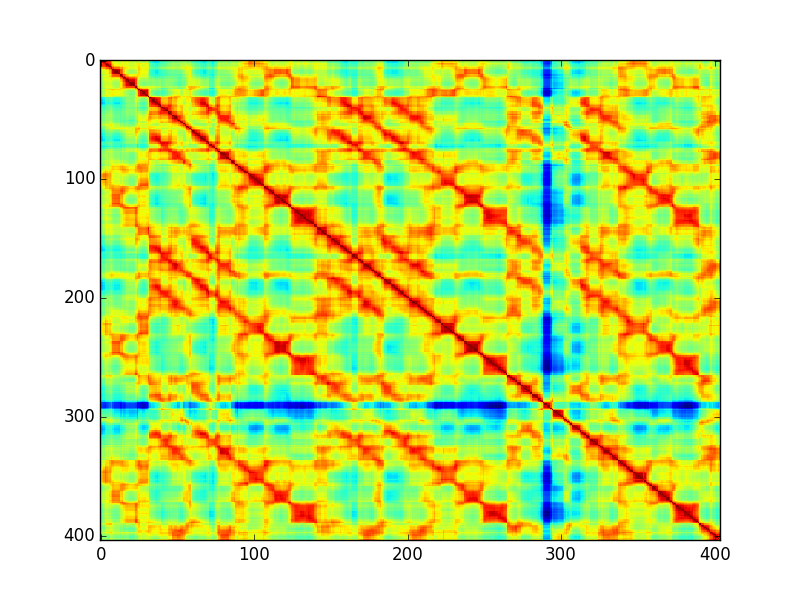
\includegraphics[width=\textwidth]{Figures/ssm_euclidean}
                \caption{Similarity matrix calculated from harmonic pitch class profiles chroma using Euclidean distance.}
                \label{fig:euclidean}
        \end{subfigure}%
        \begin{subfigure}[b]{0.31\textwidth}
                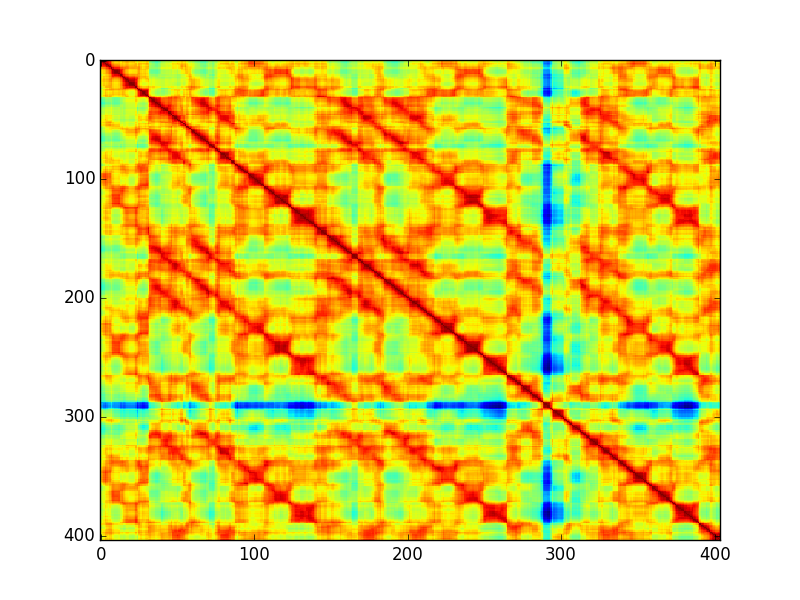
\includegraphics[width=\textwidth]{Figures/ssm_manhattan}
                \caption{Similarity matrix calculated from harmonic pitch class profiles chroma using Manhattan distance.}
                \label{fig:manhattan}
        \end{subfigure}
         \begin{subfigure}[b]{0.31\textwidth}
                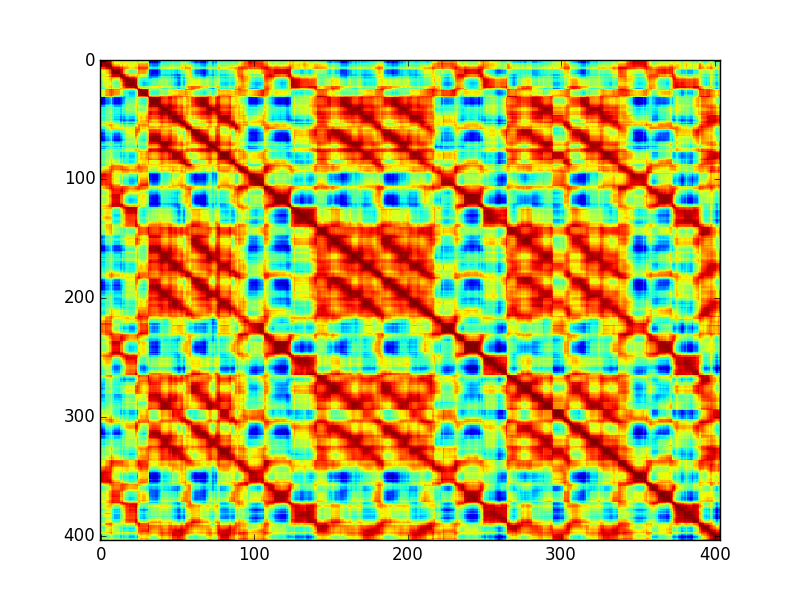
\includegraphics[width=\textwidth]{Figures/ssm_cosine}
                \caption{Similarity matrix calculated from harmonic pitch class profiles chroma using cosine distance.}
                \label{fig:cosine}
        \end{subfigure}
          \caption{Comparison of SSM computed using different distance formulas. The SSM calculated using correlation distance can be seen in Figure \ref{fig:synSSM}.}
        \label{fig:ssmdistance}
\end{figure}


When we look at the SSM computed using cosine distance, we can notice that the amount of the similar points increased, more similar to the the one generated using the correlation distance. However, the correlation distance on Figure \ref{fig:synSSM} contains more dark blue spots, implying that it exposes more beats that are, in fact, not similar. This is why, in our design of the structure retrieval of a song we decided to use SSM computed using correlation distance.

\vspace{10pt}

\begin{figure}[h]
        \centering
        \begin{subfigure}[b]{0.47\textwidth}
                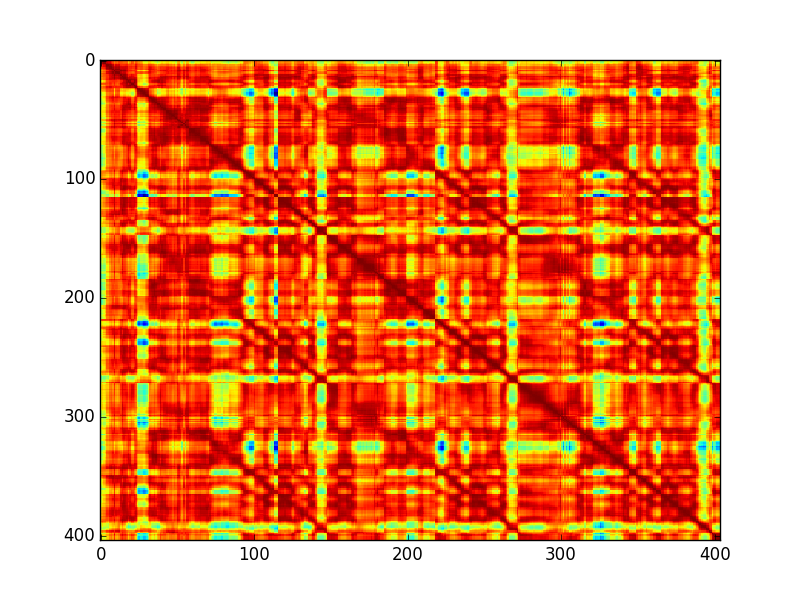
\includegraphics[width=\textwidth]{Figures/mfcc_no_log_sync}
                \caption{Similarity matrix generated from Mel-frequency Cepstral Coefficients without log normalisation.}
                \label{fig:unMFCC}
        \end{subfigure}%
        \begin{subfigure}[b]{0.47\textwidth}
                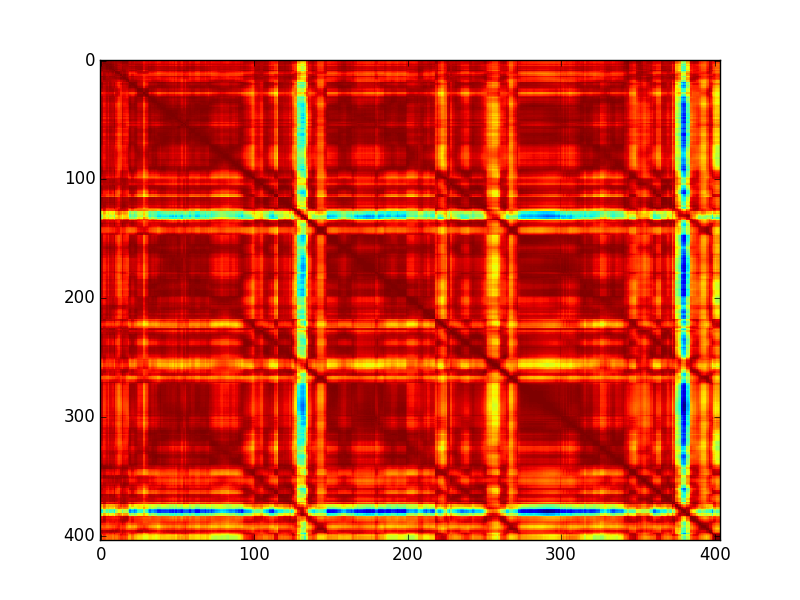
\includegraphics[width=\textwidth]{Figures/mfcc_ssm_synched}
                \caption{Similarity matrix generated from Mel-frequency Cepstral Coefficients with application of log normalisation.}
                \label{fig:synMFCC}
        \end{subfigure}
          \caption{Comparison of SSM generated from unprocessed and enhanced MFCCs, using correlation distance.}
        \label{fig:MFCCcomparison}
\end{figure}

\subsubsection*{Mel-frequency Cepstral Coefficients}


Similarly to the case of Harmonic Pitch Class Profiles, we started the preparation of the features by beat-synchronisation to decrease the size of the data for further analysis. 

Next, we had to determine whether log normalisation improved the clarity of the SSM. As we can see in Figure \ref{fig:MFCCcomparison}, the use of log normalisation could decrease the amount of segments found, as more similar points are exposed.

Finally, we computed the SSM. Again, we investigated the possibility of generating it using Euclidean, Manhattan and cosine distances. The diagrams presenting our findings can be seen in Section \ref{sec:mfccappen}, Appendix B. Similarly to when we were working with HPCPs, the correlation distance gave us the most contrasted, sharper images. 

The result of this process can be seen in Figure \ref{fig:synMFCC}.

\vspace{10pt}

\subsection{C-NMF}


\begin{wrapfigure}{r}{0.5\textwidth}
\vspace{-20pt}
  \begin{center}
    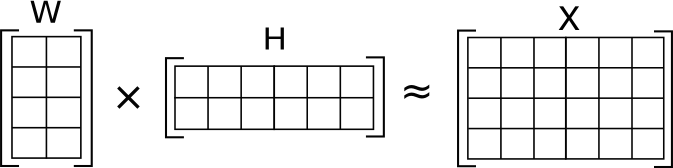
\includegraphics[width=0.45\textwidth]{Figures/NMF}
  \end{center}
  \caption{Illustration of approximate non-negative matrix factorization: the matrix $X$ is represented by the two smaller matrices $W$ and $H$.}
\label{fig:NMF}
\end{wrapfigure}

We can view the SSM as an array of column vectors where each vector corresponds to a window. Suppose we have a set of vector templates. Vectors in the steady regions of a song may be directly found in the set, while vectors in the boundary regions may be approximated by linear combination of vector templates. Making this observation, we believe the Non-negative Matrix Factorization (NMF) could be useful in our situation.

In NMF, the $N \times N$ self similarity matrix $X$ is approximately factorised into product of a $N \times k$ matrix $W$, can be interpreted as a cluster row matrix, and $k \times N$ matrix $H$, composed of the indicators of these clusters, where $k$ is the rank of the composition. This can be described as $X \approx WH$. The $j$th column of $W$ can be viewed as the vector template for the $i$th segment type. The $j$th column of $H$ describes the intensities of the $k$th segment types for the $j$th window. In NMF, both $W$ and $H$ are enforced to be positive (i.e. $X$ must be positive too). We denote a row vector by $\boldsymbol{z}$ and a column one by $\boldsymbol{z}^{T}$.

However, in data mining, sometimes it can be beneficial to ensure $X$ to contain meaningful “cluster centroids”, i.e., to restrict $W$ to be convex combinations of data points.
C-NMF adds a constraint to $W$ = ($\boldsymbol{w}_{1}^{T}$, $\boldsymbol{w}_{2}^{T}$,... ,  $\boldsymbol{w}_{k}^{T}$),  such that its columns  $\boldsymbol{w}^{T}$  are, in fact,  convex combinations of the features of $X$:

\begin{equation}
\boldsymbol{w}_{j}^{T} = \boldsymbol{x}_{1}^{T}f_{1j} + \boldsymbol{x}_{2}^{T}f_{2j} + ... + \boldsymbol{x}_{N}^{T}f_{Nj}  \hspace{45pt}   j \in [1 : k]
\end{equation}

The linear combination is convex if all coefficients $f_{ij}$ are positive and the sum of each set of coefficients  $\boldsymbol{f}^{T}_{j}$ must be 1. Formally, this can be represented as:
$f_{ij} \geq 0,  f_{ij} = 1 $

This results in $W = XF$, where $F \in \mathbb{R}^{N \times k}$, which makes the rows $\boldsymbol{f}_{i}$ interpretable as weighted cluster centroids. The decomposition matrices $R_{j}$, are obtained as follows:  $R_{j} =  \boldsymbol{w}^{T}_{j}\boldsymbol{h}_{j}$, where $j \in [1 : k]$. Finally, C-NMF can be formally characterised as: $X \approx XFH$.

In C-NMF, the matrix $W$ is a set of convex combinations of the rows of the input matrix $X$, which contrasts with NMF, where no such constraint exists. This means that, each row $x_{i}$ represents similarity of the time frame $i$ with the rest of the time frames, storing information about the time frame $i$ across the entire song.

By computing the C-NMF we separate basic structural parts. In the next section, we describe how the factorization via C-NMF relates to structure and show how we can use that result for music structure discovery. 

Apart from this, another important benefit of C-NMF over NMF is that matrices $W$ and $H$ become naturally sparse when adding the convex constrain. In case of NMF the $H$ does not always become sparse. Thanks to that, when using C-NMF we are more likely to find similar decomposition matrices for the same input than NMF, which is more sensitive to its initialisation \cite{Nieto}. 

\vspace{10pt}


\subsection{Boundaries}

\begin{figure}
        \centering
        \begin{subfigure}[b]{0.47\textwidth}
                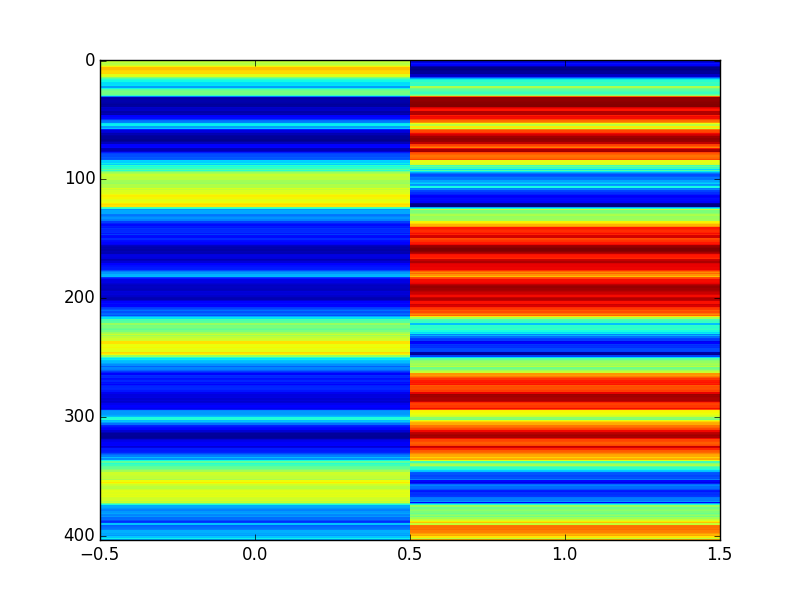
\includegraphics[width=\textwidth]{Figures/F}
                \caption{The cluster matrix $W$.}
                \label{fig:Wmatrix}
        \end{subfigure}%
        \begin{subfigure}[b]{0.47\textwidth}
                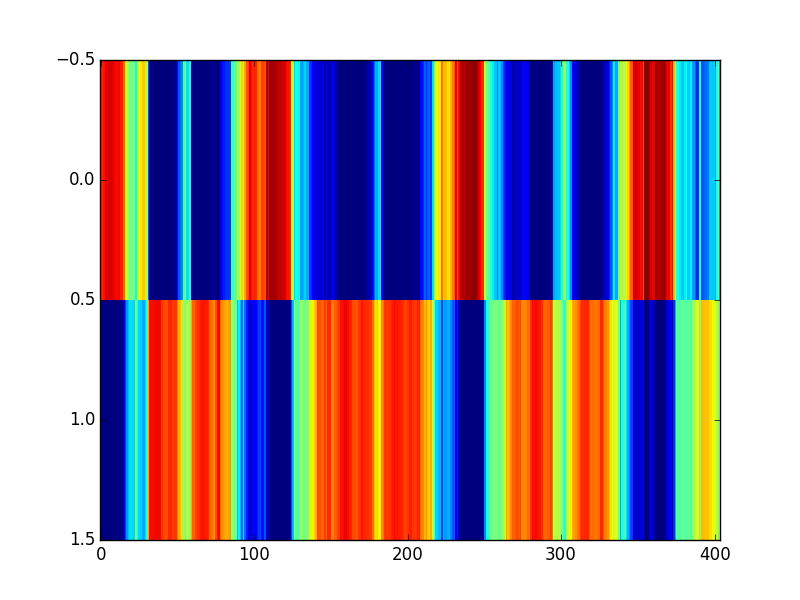
\includegraphics[width=\textwidth]{Figures/G}
                \caption{The activation matrix $H$.}
                \label{fig:Hmatrix}
        \end{subfigure}
          \caption{The result of C-NMF computed for ``Help!'' by The Beatles with rank $k = 3$.}
        \label{fig:CNMFbeatles}
\end{figure}
 
In this section we will investigate different ways of obtaining section boundaries from the decomposition matrices obtained from applying C-NMF to the similarity matrix. An example of resulting cluster and activation matrix computed with C-NMF with rank $k = 2$ can be seen in Figure \ref{fig:CNMFbeatles}.

\subsubsection*{Pure C-NMF Approach}
\label{sec:finalBounds}

Clustering is an unsupervised classification of patterns, for example observations, data items, or feature vectors, into groups called clusters. The points within each cluster should be similar to each other and dissimilar to points belonging to another cluster. The problem has been addressed in many contexts and by researchers in many disciplines.

Having applied the C-NMF, we computed, we have generated two decomposition matrices - $W$, called the cluster matrix, and $H$, an activation matrix, so that by multiplying them we can recreate the SSM, ie. $X \approx  WH$       
        
To obtain the boundaries, we filter both the cluster matrix $W$ and the activation matrix $H$. This means that for every row corresponding to a frame in which the beat occurs, we find the indexes of the its maximum values. Thanks to this simple clustering, we obtain a assignment of each of the frames to one of the 'types' of segments. By iterating through a matrix generated and such ways and recording the indexes at which a song changes from one portion to another, we manage to obtain section boundaries in an efficient way. In our implementation, we start the computation with rank $k = 3$ and increase it if not enough bounds were found. This is to avoid overfitting and creating tiny segments, for example, one per verse line.

Once we have boundaries, we combine them within a distance window of size h so that boundaries close to each other get merged in their average location.

This method, although quite simple, produced a neat and quite accurate output, with a few, but meaningful segments. In the next section we describe an attempt of improving our results that did not yield results we hoped for, and hence was left out in the final implementation.

\subsubsection*{K-means Clustering}
\label{sec:kmeans}

\begin{figure}[b]
        \centering
        \begin{subfigure}[t]{0.30\textwidth}
                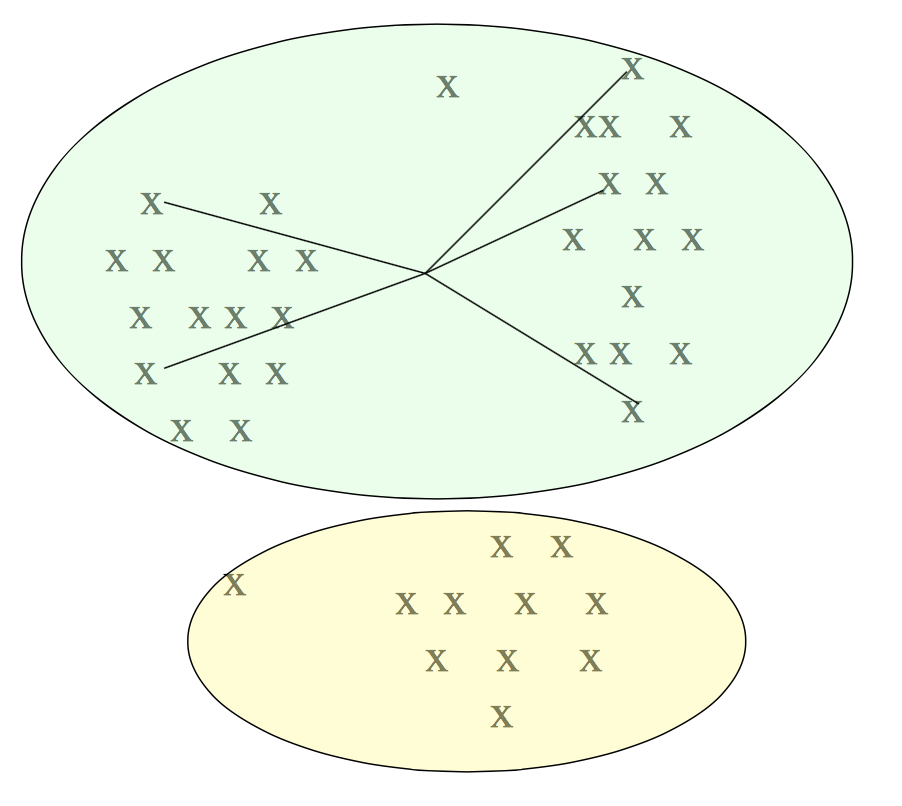
\includegraphics[width=\textwidth]{Figures/underfitting}
                \caption{The k value is too small - many long distances to centroids.}
                \label{fig:underfitting}
        \end{subfigure}%
        \begin{subfigure}[t]{0.30\textwidth}
                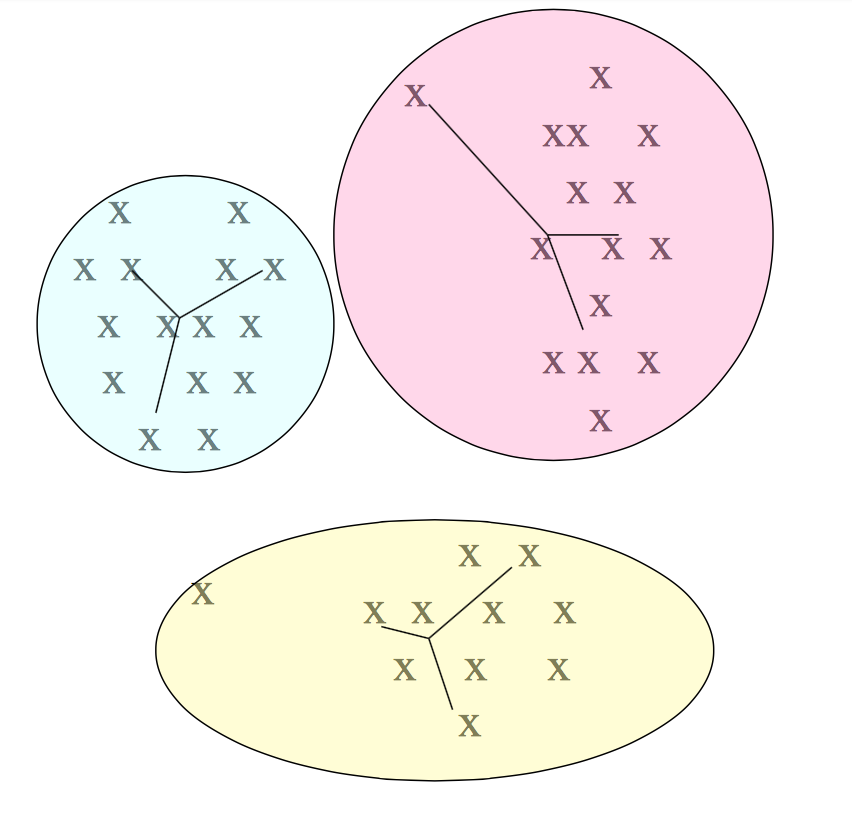
\includegraphics[width=\textwidth]{Figures/justright}
                \caption{Good k value - distances to centroids are quite short.}
                \label{fig:justright}
        \end{subfigure}
         \begin{subfigure}[t]{0.30\textwidth}
                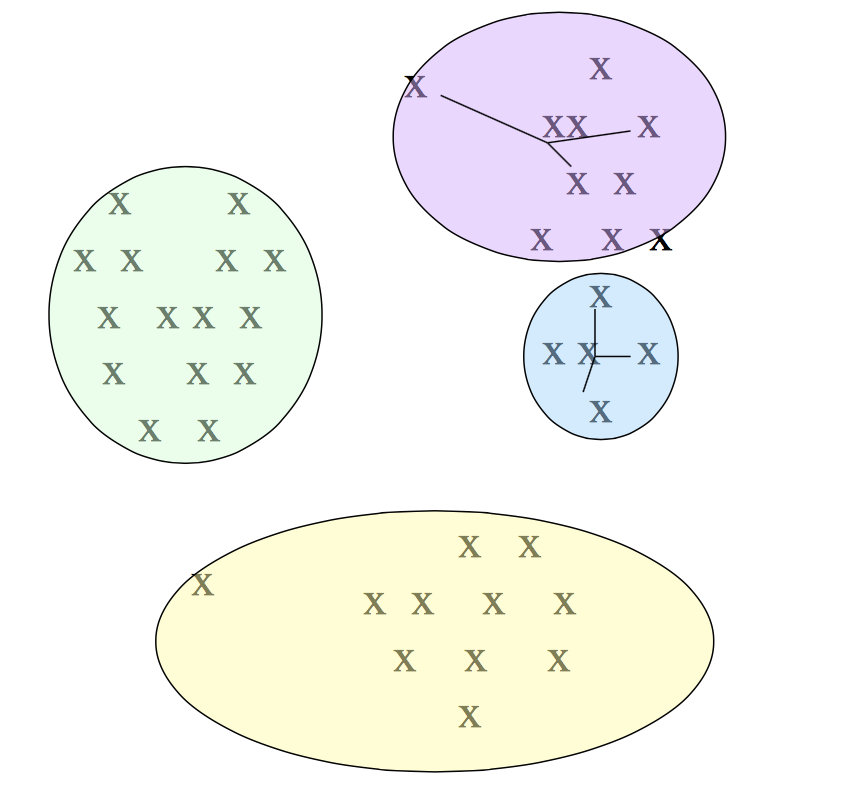
\includegraphics[width=\textwidth]{Figures/overfitting}
                \caption{The k value is too big - little improvement in average distance.}
                \label{fig:overfitting}
        \end{subfigure}
          \caption{Diagrams depicting impact of the $k$ value on the clustering result \cite{kcluster}.}
        \label{fig:kmeansclustering}
\end{figure}

K-means clustering is considered one of the simplest unsupervised learning algorithms that can solve the well know clustering problem. It follows a simple and easy way of classifying a given data set through a certain number of clusters (assume $k$ clusters).

The main idea  is to define $k$ centres, one for each cluster. Much care should be put into their placement, as different location of centres causes different result. This is why the most intuitive solution is to put them as far apart as possible. The next step is to take one point after another from the data set and associate it with the nearest centre, 

When all the points have been assigned to some centre, $k$ new centroids are calculated as baycentres of the clustering that resulted from the first phase. Once we have calculated the new centroids, a new binding has to be done  between the same data set points and the nearest new center. Very often this will result in points moving between different clusters. This can be considered second phase of the algorithms. 

Those two phases are repeated in a loop. As a result, we may notice that the $k$ centers change their location step by step until no more changes are done, and the algorithm converges. 

We ran k-means clustering with $k = 2$ to each one of the C-NMF decomposition matrices, interpreting them as row-vector features. We efficiently obtained the section boundaries The choice of $k = 2$ allows us to detect boundaries (i.e. there’s a boundary or not), regardless of how the various sections cluster. However, after comparing the output of an this algorithm with a manually created segmentation, we noticed that k-means clustering's performance was not suited for our use. The granularity of the segmentation was too high - very often it separated parts of verse, or even fractions of seconds. Even after merging values that were close together and getting rid of the smallest segments, the boundaries detected were too granular.

\vspace{10pt}


\subsection{Labelling}

In our structure retrieval, we investigated different ways of labelling of the segments.

First approach built directly on our way of segmenting the song.
Similarly to when attempting to find boundaries between segments, we decomposed our self similarity matrix $X$ with rank increased. This allowed further differentiation between structures, for instance, if certain part of a song was thought of as a chorus, but it is different enough to get separated in a C-NMF of a higher rank.

Once we have decomposed the matrix $X$, we filtered the clustering matrix $W$, as described in Section \ref{sec:finalBounds}. This way, we computed initial clustering for each beat frame. To synchronise labels calculated in such way, we assigned a numerical label which occurred within each of the interval between two segment to them.

\begin{figure}[h]
	\centering
   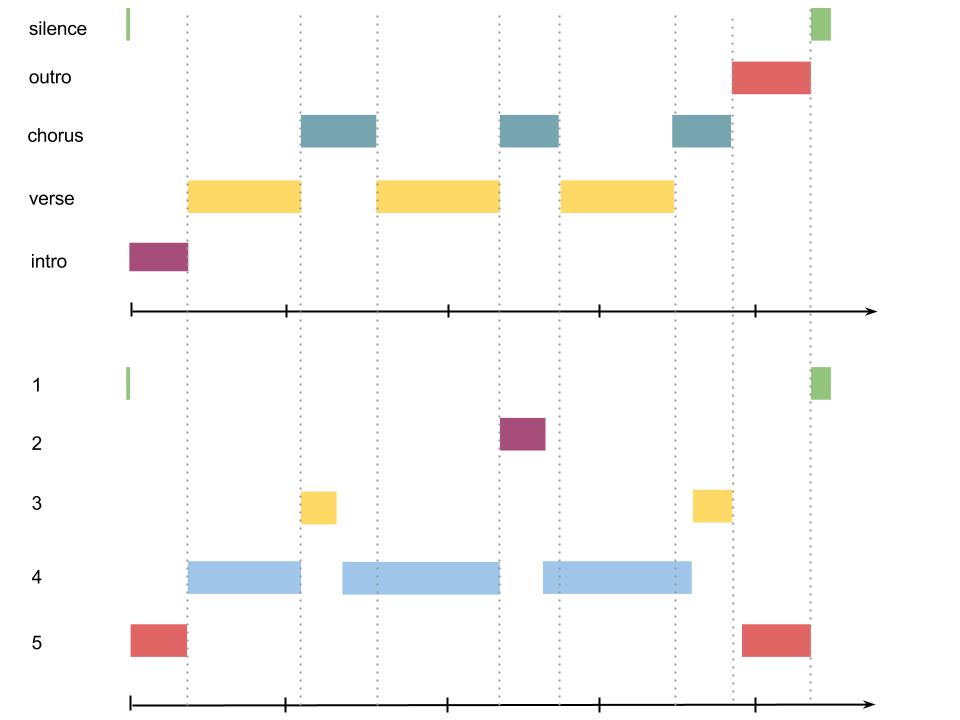
\includegraphics[width=0.7\textwidth]{Figures/NumericalLabels}
\caption{A depiction of the pure vocals detection as a labelling method (bottom) compared with manual segmentation and labelling (top).}
\label{fig:numericsimple}
\end{figure}

However, ideally in our application we would like to be able to tell the player what segment he is currently in and make them as clear and easy to understand as possible. As we could not find literature where this was attempted, we had to investigate various ways of achieving this ourselves. 

Having gathered data about the main melody of the song earlier on, we could use it to more accurately predict the labels for each of the song segments, producing labels that easy to understand to a person. 

In attempt to do so, we synchronise the array of pitches with the beats to get beat synchronised features which we could with ease refer to once we have the boundary frames. 

\begin{figure}[h]
	\centering
   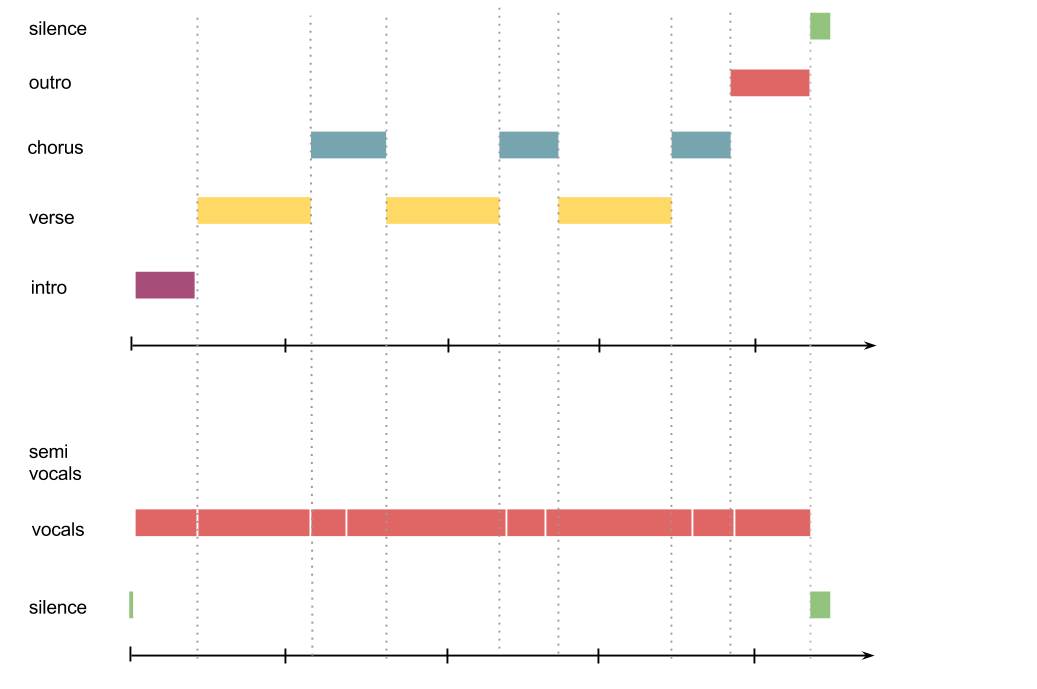
\includegraphics[width=0.7\textwidth]{Figures/BeatlesSegmentation}
\caption{A depiction of the pure vocals detection as a labelling method (bottom) compared with manual segmentation and labelling (top).}
\label{fig:vocalsimple}
\end{figure}

First intuition we had was to investigate the amount of silent frames occurring in each of the segments. We designed heuristics to decide whether the segment we look at is vocal (majority of the frames contain the main melody), semi-vocal (the same amount of frames that are contain the main melody and not), instrumental (minority of the frames contain the main melody) or silent. 

A visualisation of our segmentation and labelling using only vocal/instrumental heuristics which can be seen on Figure \ref{fig:vocalsimple}. The diagram makes it evident that our boundary finding works quite well. As we can see, each beginning of the chorus is detected with high accuracy. Moreover, the beginning and the end of the intro and outro parts are predicted really well. In addition to this, the segmentation process manages to detect the silence segments in the beginning and end of track. However, our clustering algorithm detects the end of the chorus too early, absorbing a part of it into the verse that follows.

\begin{wrapfigure}{r}{0.5\textwidth}
\vspace{-30pt}
  \begin{center}
    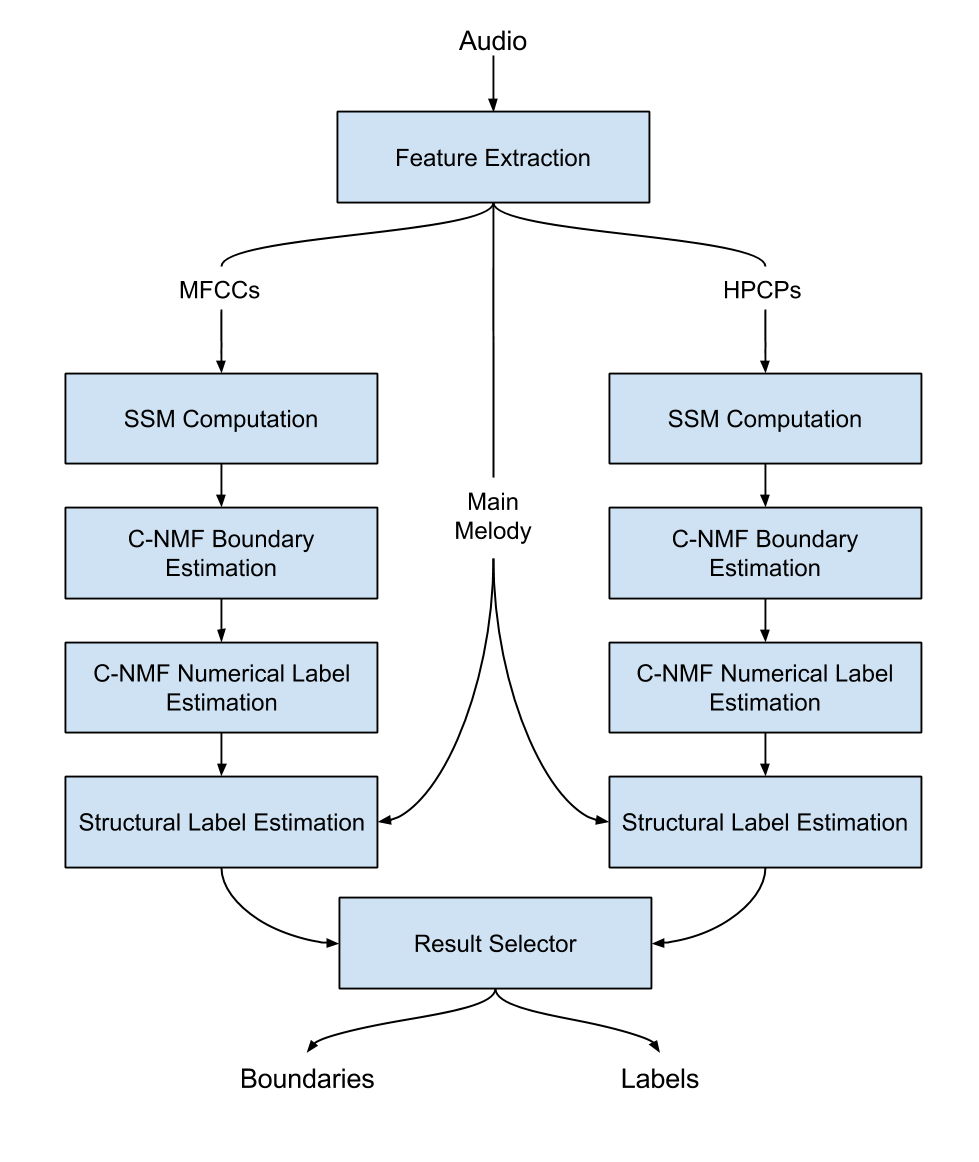
\includegraphics[width=0.48\textwidth]{Figures/Structure-Retrieval}
  \end{center}
  \caption{Depiction of the final design of our structure retrieval system.}
\label{fig:NMF}
\end{wrapfigure}

However, this way alone, we lose the distinction between the vocal parts, for instance, between the verse and the chorus. We could implement a system of heuristics to assign labels like chorus or verse, but unfortunately there is no straightforward way of doing so as the song structures differ greatly across the popular music. For instance, many songs drop the verse-chorus structure to start with a chorus, like ``She Loves You'' by The Beatles.

Our final approach was to merge the two approaches mentioned earlier into one algorithm. Ideally, we wanted to preserve the variation in the vocal parts, as it was presented in the first approach where multiple parts were classified with the same class, while being able to tell when the main melody of is present, and when it is not. Moverover, we had to find a solution to the problem of determining which segments contain chorus, which ones represent the verse and which should be classified otherwise.


To make it possible, we first employed our initial labelling algorithm to retrieve numerical labels for each of the detected segments. This way we were able to find relationships between different segments. Once we know which segments bear high similarity, we average the amount of percentage of voiced frames per segment. Having done that, we look at the two most repeated segments. The one with the higher average of the voiced frames is labelled as a chorus, and the other one is determined to be a verse. The first segment is labelled an intro if it bears not similarity to other segments. If it is classified the same way the last segment is, we label both if them as "intro/outro". If our algorithm finds another segment similar to any of them, they are marked as the bridge.

\vspace{10pt}


\subsection{Final Design}

Once we have designed the the labelling algorithm, we researched the impact of the choice of feature on the performance of the segmentation. We had noticed that some songs achieved better results when HPCPs were chosen to lead the computation and retrieve the song segmentation whereas the others performed better with MFCCs taken into account. 

To solve the dilemma of the choice of feature, we implemented a selector, which inspecting the outputs produced using HPCPs and MFCCs, selects the one which is most likely to reflect the structure of the song. It investigates boundaries and labels returned by processing each of the SSMs and looks at their structure - the length of the silences, length amount of segments detected and how the segments fit into their neighbourhood. Based on those observations, it ranks both outputs based on their likelihood and selects the most likely one. 


\vspace{20pt}


\section{The Game}

In this section, we will go over the architecture and the design choices made when planning and implementing our game.

The game is written mostly in Swift, a multi-paradigm, compiled programming language created by Apple Inc. for iOS and OS X development. 
It was first introduced at Apple's 2014 Worldwide Developers Conference (WWDC). Swift is designed to work with Apple's Cocoa and Cocoa Touch frameworks, building on the best of C and Objective-C, without the constraints of C compatibility. It adopts safe programming patterns and adds modern features to make programming easier, more flexible, and more fun \cite{swiftintro}. 

We chose this language as we wanted to create a game for the OS X platform. In addition to this, the author also had a personal interest in learning the language.

For the music analysis part of the project we used Python. This is because there are many libraries available in this language for both training of artificial neural networks and music analysis. 

\vspace{10pt}


\subsection{Data Storage}

The game relies on preserving user's scores and the levels generated by them. We need a way of storing them and all the information retrieved when analysing the songs to avoid regenerating the levels for the same song, for example if the user has a music piece they particularly like.

Core Data is the standard way to persist and manage data in both iPhone and Mac applications. It is an object graph and persistence framework provided by Apple in the Mac OS X and iOS operating systems. 

Core Data describes data with a high level data model expressed in terms of entities and their relationships plus fetch requests that retrieve entities meeting specific criteria. Code can retrieve and manipulate this data on a purely object level without having to worry about the details of storage and retrieval. 

\begin{wrapfigure}{r}{0.5\textwidth}
  \begin{center}
    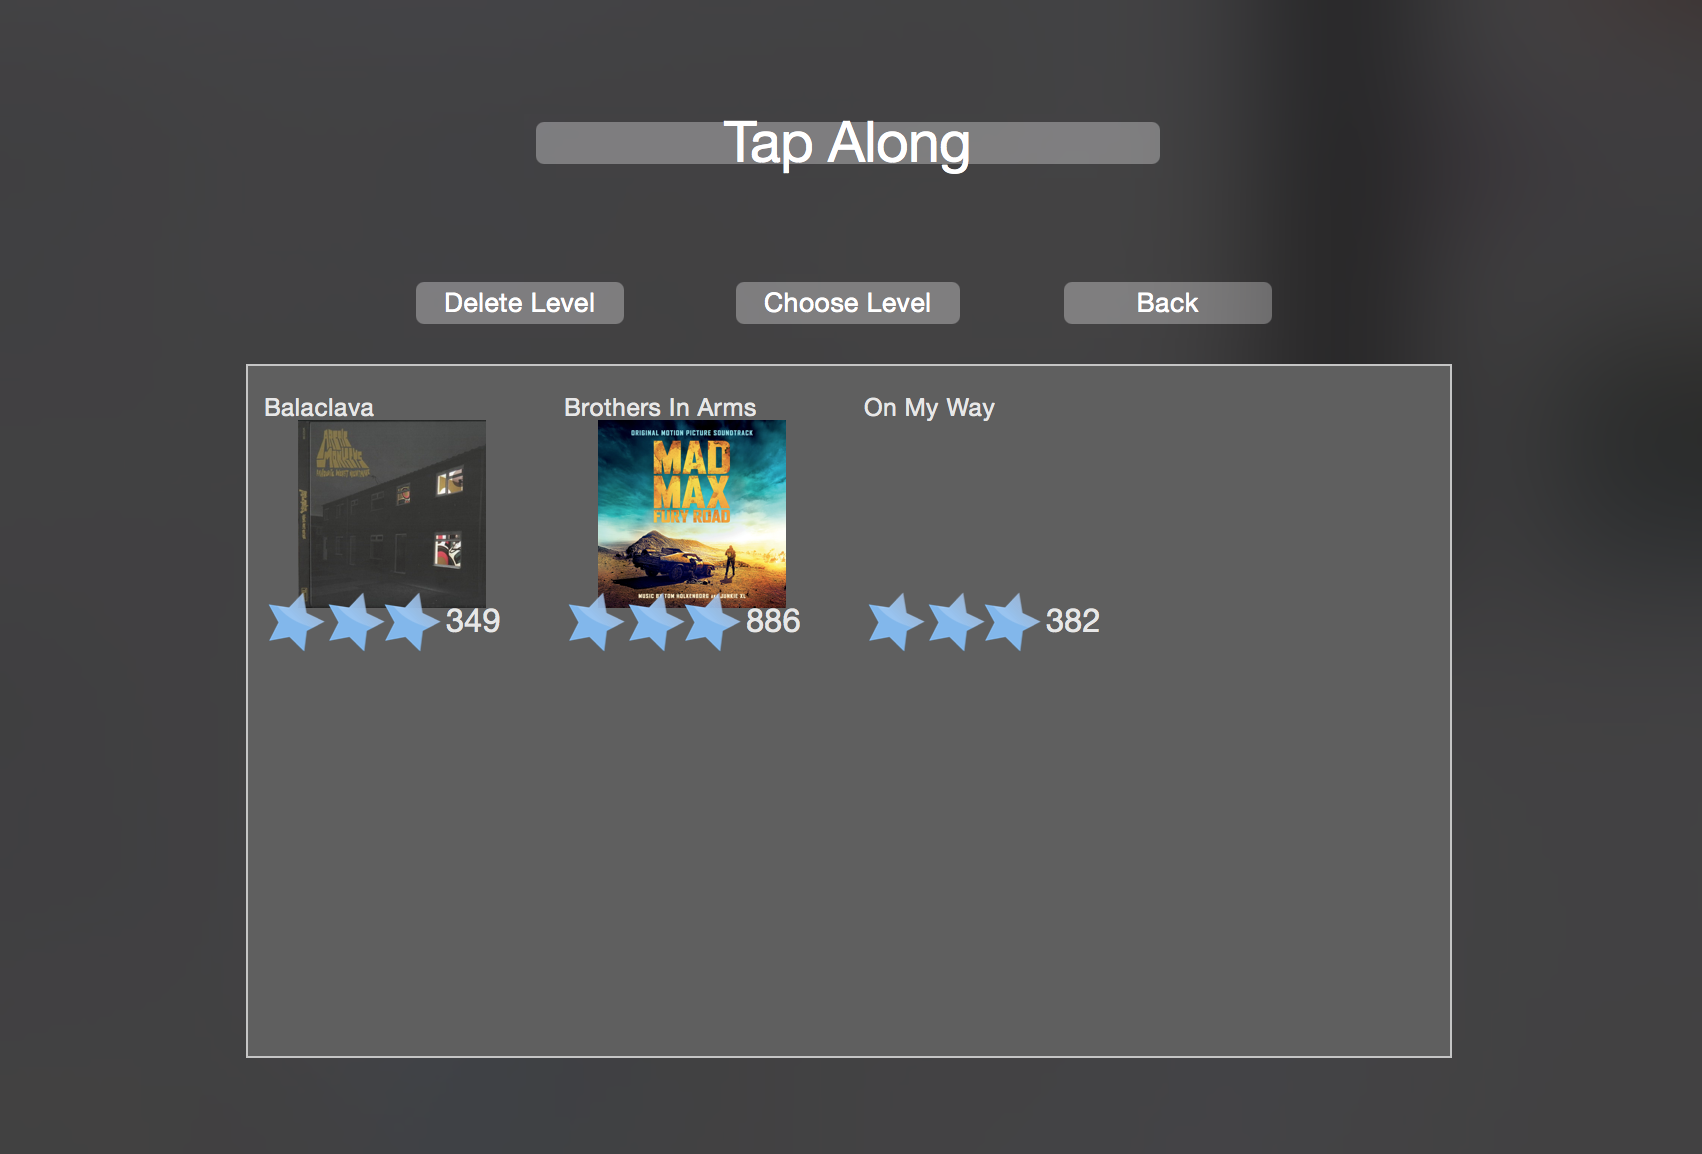
\includegraphics[width=0.45\textwidth]{Figures/CollectionView}
  \end{center}
  \caption{Screenshot of the game in the song selection menu.}
\label{fig:songselection}
\end{wrapfigure}

Core Data allows data organised by the relational entity–attribute model to be serialised into XML, binary, or SQLite stores.

Core Data is also a persistent technology, in that it can persist the state of the model objects to disk. But the important takeaway is that Core Data is much more than just a framework to load and save data - it is also about working with the data while it is in memory.
We decided to use Core Data rather than a separate database as our game only needs to store data used by the current user, that will be utilised almost immediately after loading into memory. 
  
The model might cause some intensive memory usage if we decide to create a big amount of users, however, as it is an offline game that can be played on a personal machine, in contrast to web application, the number of users should remain relatively small.

\vspace{10pt}

\subsection{Menu}

Although not usually adopted in OS X games, we decided to follow the Model-View-Controller design pattern in implementing our application. We believe it was a right choice as the complexity of the main menu would have to be then supported throughout the played level. This would not only be a performance strain, but would also cause the code to be messy.

When first facing the menu, the user has an option of creating an account, logging in as a user or playing a quick game, not requiring any user data. 
The quick game is essentially an ability of playing one of the predefined levels, without a choice of creating a new one.

Once the user has created an account or chosen an existing one, they can either follow the level creation or level loading option. If they choose to create a new level, they have to select a file from their hard drive they would like to use as the base for their level. Otherwise, they go to the window, where they can select a level and either play it or remove it from their catalogue.

To design the song selection view, we made use of the \verb|NSCollectionView|, which allows to display objects in a grid. Each view in the grid is represented by a \verb|NSCollectionViewItem| object, which manages the loading of the view's content.

Each element in our collection view contains the name of the level, the artwork of the song it was based on extracted from the ID3 tags of the file, the maximum amount of the points scored and the stars awarded for the score. The design of the song selection menu can be seen in Figure \ref{fig:songselection}

\vspace{10pt}

\subsection{Song Description}

Once we move on to playing a game, the \verb|GameViewController| unpacks the \verb|GameScene| - an object representing a scene of content in Sprite Kit.

\begin{wrapfigure}{l}{0.5\textwidth}
  \begin{center}
    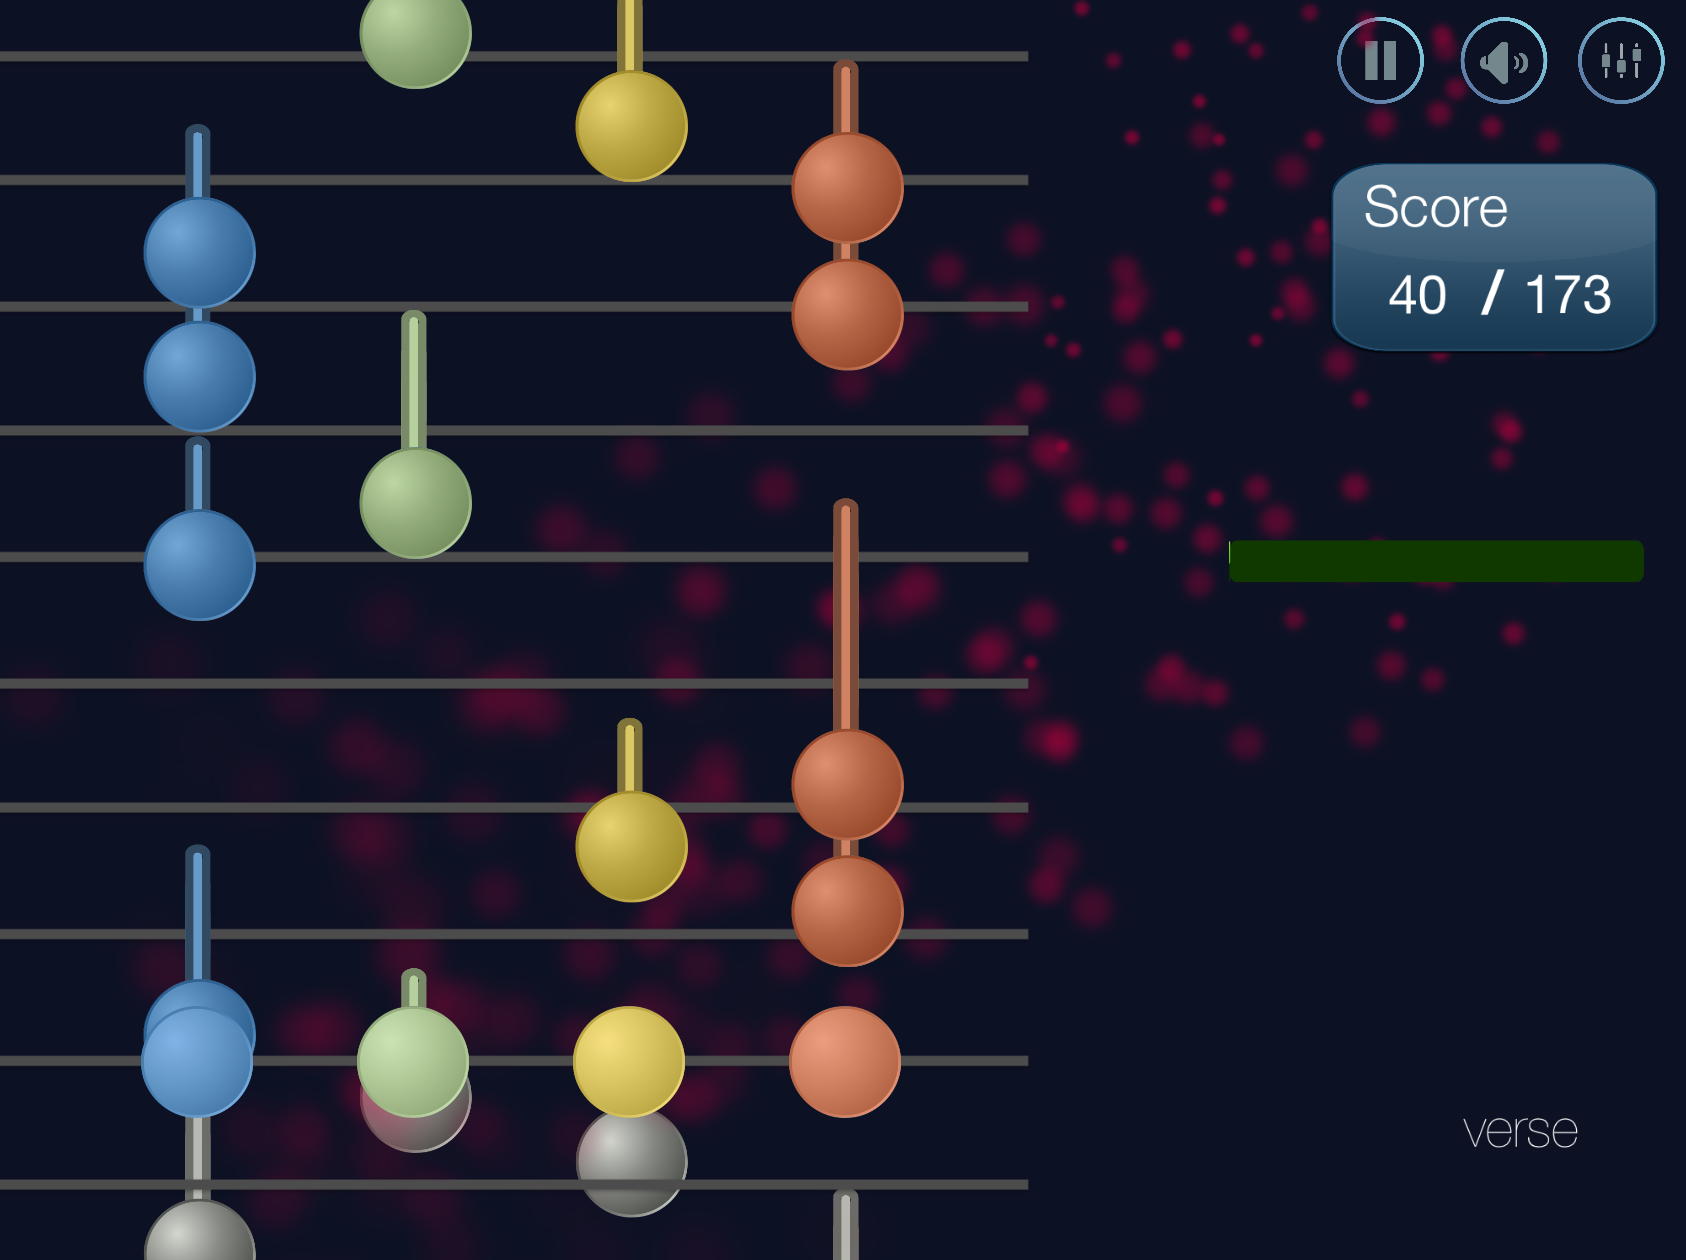
\includegraphics[width=0.45\textwidth]{Figures/FullGame}
  \end{center}
  \caption{Screenshot of the game in the middle of playing a song.}
\label{fig:overallgamescreen}
\end{wrapfigure}

Sprite Kit provides a graphics rendering and animation infrastructure that can be used to animate arbitrary textured images, or sprites. It uses a traditional rendering loop where the contents of each frame are processed before the frame is rendered. Its advantage is that it was developed for Apple hardware, hence it is optimised to render frames of animation efficiently using the graphics hardware. Thanks to this, the positions of sprites can be changed arbitrarily in each frame of animation. Sprite Kit also provides other functionality that is useful for games, including basic sound playback support and physics simulation. \cite{spritekit}. 

In the game scene, there is a set of buttons at the bottom of the screen. Players use the strum bar along with the fret buttons to play notes that scroll down the screen. The Easy difficulty only uses the first three fret buttons, that is, the green, red, and yellow. The Medium difficulty uses the blue button in addition to those three, and Hard and Expert use all five buttons.

The score is calculated based on how many scrolling notes we manage to hit. Every time we hit, the performance bar on the right side of the screen goes up, otherwise it goes down. If it hits the minimum, it the player loses. However, if the player manages to keep the performance level at the maximum for an appropriate amount of time, the number of the points scored for the new notes gets doubled until he misses a note or wins the song.

The player can at any time pause, stop or replay the game. They can also control the volume of the music and other sounds in the game. 

Upon completion of the level the player presented with their score, shown as stars and a concrete number. The player can later revisit the songs if they want to improve their score. 

\vspace{10pt}

\subsection{Melody Detection as a Game Changer}

The main part of the gameplay relies on the user pressing buttons that line up on the screen. As this is a music game, there are various ways of making the process more intuitive and hence attractive to potential players. 

One of the possibilities is to use the main melody of the song to determine which buttons to issue for the player by tying in the melody extraction. In particular, by creating a mapping between the pitches and the buttons that need to be pressed that would somehow be similar to the way people play the musical instruments would be useful.

The main idea of the game is to mimic the playing an instrument on the computer keyboard. For this purpose we looked to 2 most popular instruments - guitar and piano for inspiration. 


When playing the piano, we are presented with a set of keys. The further to the right we press the key, the higher the note played. And likewise, if we press some key to the left, the pitch we hear is of lower frequency. 

\begin{wrapfigure}{r}{0.5\textwidth}
  \begin{center}
    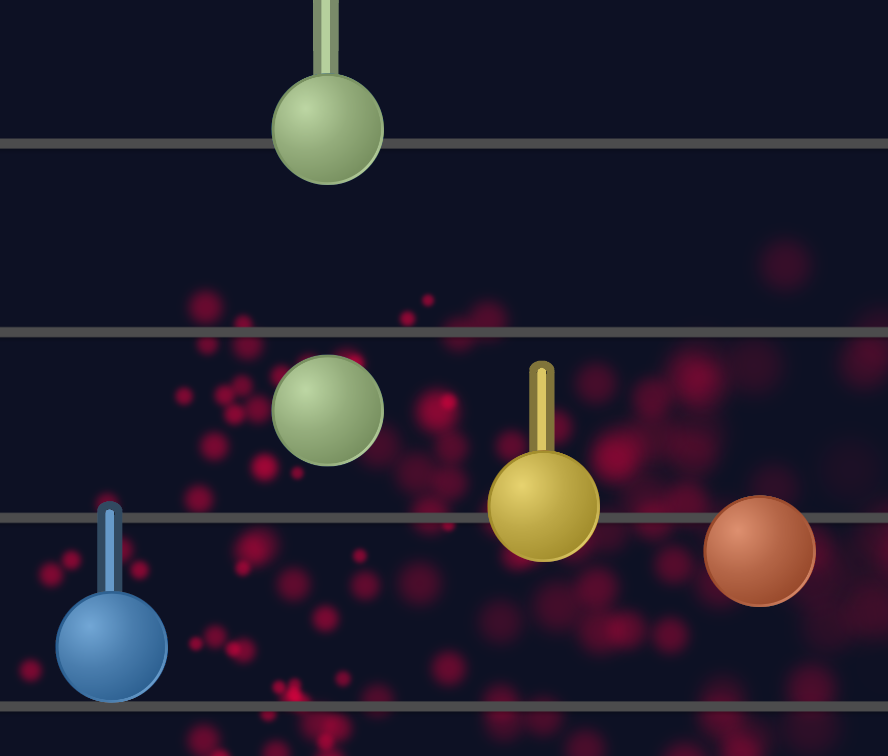
\includegraphics[width=0.45\textwidth]{Figures/NotesComing}
  \end{center}
  \caption{Screenshot presenting different types of notes approaching.}
\label{fig:notetypes}
\end{wrapfigure}

A similar, but slightly modified rule applies to the guitar. It is still true that jumping one way from one string to another increases the fundamental frequency heard and decreases it if we move back. However, another way of "going up a tone" is to go up a fret (i.e. closer to the sound hole). When we play the guitar, going up a certain amount of frets of on one string might let us play higher notes on it than other string whose fundamental note is much higher. 

This inspired us to design our notes system in a round robin fashion. If the fundamental frequency of the frame we are about to play is higher than the one we just played, the note should appear to the right of it, if lower then to the left, and if the fundamental frequencies are the same, the button should appear at the same relative position in the $x$ axis. 

However, if we need to move the note higher but we have hit the limit given by the difficulty of the song, we generate the position in a round-robin fashion, inspired by 'going up a few frets' as it is a case with the guitar.

Another interesting feature to work on was the length of the notes. To increase the difficulty, every time we detect a longer note - i.e. a repeated notes of the same frequency, instead of adding a button per note, we make the note longer, as it can be seen in Figure \ref{fig:notetypes}.

\vspace{10pt}

\subsection{Introduction of the Song Segmentation}

One of the features that clearly distinguishes this project from other rhythm based games, apart from using the estimated main melody to generate the gameplay, is the use of automated music track segmentation. We aimed to use it to guide the user through the song - to indicate similar elements of the song or simply let the users know how far along in the song he is. 

To achieve that, we dedicated a part of the screen to indicate the user of their progress within a song. Every time the player moves on to the next segment of the song, its label shows in the bottom left screen.

\vspace{10pt}

\subsection{Impact of the Mood on the Level}

\begin{wrapfigure}{r}{0.5\textwidth}
  \vspace{-10pt}
  \begin{center}
    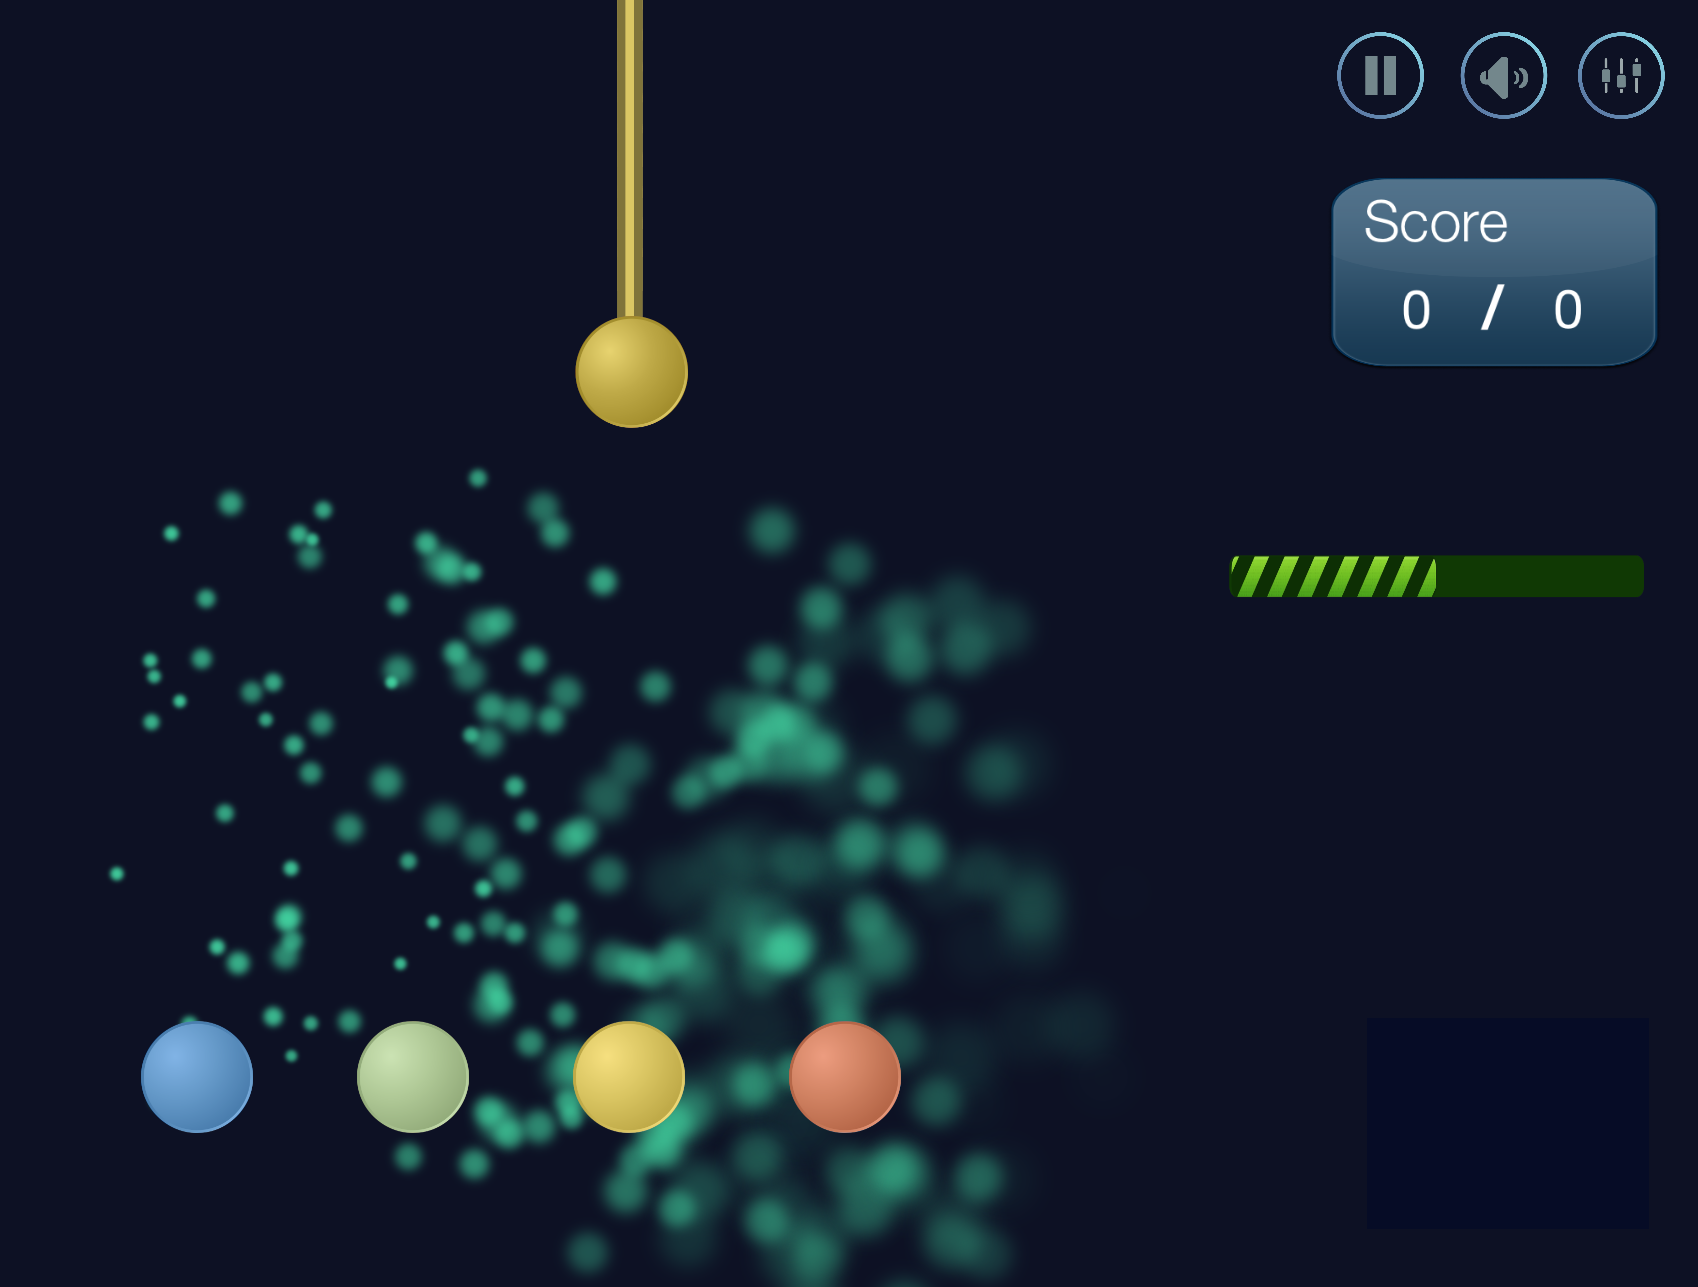
\includegraphics[width=0.45\textwidth]{Figures/sparkChange}
  \end{center}
  \caption{Screenshot showind the song at the beginning of the musical track, when the main melody is about to play, with a mood completely different from the one depicted in Figure \ref{fig:notetypes}.}
\label{fig:notetypes}
\end{wrapfigure}



Once we have implemented and introduced the song segmentation, it was time to create the environment that would be affected by the mood in the song.

One of the features of music which can indicate the changes in emotions in a song can be the beats. If the beats are fast, more frequent, the song sounds more energetic, whereas a phlegmatic song will have softer, slower beats. 

To aid the players with the game, we introduced ``frets'' coming down the screen together with the notes. They allow the user to ``place'' the note within the tact, aiding him to ace it. Due to possible variation in beat intervals, in implementing this feature we had to make use of timers that constantly check the time between the two next beats. This caused some problems when implementing the pause in the game, but they were overcome by storing the state of the timers once the pause is hit and recreating the timer once the game is resumed with it. 

Now we are ready to use our neural network for the mood detection. For every segment detected by our system, we extract the features we found had the biggest impact on the mood perceived and activate our network on them. 

Finding a way of making the arousal and valence values have an impact on the surroundings in the game proved to be an interesting challenge in terms of usability. This is why we came up with a system where when the user creates a level, he can choose one of the two options -- subtler and more evident mood projection. In the subtle version, the user is presented with a set of particles or sparks that float around in the background. The spark's behaviour is triggered by the beat frequency, the more frequent they are, the more dynamic the moves. On the other hand, the size of the particle set as well as the colour are adjusted based the arousal and valence colour.

However, if the user opts for the second option, they are presented with much more evident changes. Apart from the particle set moving around, they can now observe the changes in the whole colour scheme of the game. This makes the influence of the mood much more evident, however it might distract, or even confuse some of the users, especially the beginners. That is why we decided to make this feature adjustable and leave it up to the user to include it or not based on their confidence in their own skills. 

